% =====================================================================
%  companion_categorical  --  STANDALONE THEORY PAPER
%  ---------------------------------------------------------------
%  Role:       full, self-contained development of the categorical
%              and homotopy-theoretic framework for viability-
%              weighted curvature: the SAVGS object, the 2-category
%              StCon(B) of stratified connections with the gluing
%              theorem and the piecewise-holonomy formula, the
%              Fisher-minimal transport law on constant-active-set
%              strata, the Bregman--Noether correspondence, the
%              seven-optic composition theorem with per-optic
%              Lipschitz constants and the Banach contraction, the
%              filtered-colimit construction of RAF sets, and the
%              HoTT/infty-categorical extension.
%  Relation:   the application paper (journal_manuscript_v2.tex)
%              states the load-bearing definitions of this
%              framework in brief adapted form and cites this
%              development for the constructions and proofs; this
%              paper cites the application paper where the empirical
%              line is concerned. The two papers share no verbatim
%              passages of length, and each is self-contained for
%              its own claims.
%  Provenance: the mathematical content descends from the frozen
%              predecessor manuscript (journal_manuscript.tex; the
%              complete source and its Git history remain committed
%              as the audit baseline). Section-level disposition
%              records live in the repository worklog and the
%              content-loss scan artifacts, not in this paper.
%  Honesty:    proof status is labeled per theorem: complete proofs;
%              proofs that reduce to cited descent/coherence theory
%              (marked); proof sketches (marked); machine-verified
%              statements with committed artifacts. Conjectures stay
%              conjectures.
% =====================================================================
\documentclass[11pt,a4paper]{article}

\usepackage{amsmath,amssymb,amsthm}
\usepackage{mathtools}
\usepackage{mathrsfs}
\usepackage[margin=2.4cm]{geometry}
\usepackage{microtype}
\usepackage{booktabs}
\usepackage{tabularx}
\usepackage{enumitem}
\usepackage{xcolor}
\usepackage{graphicx}
\graphicspath{{./}{../download/}}
\usepackage[colorlinks=true,linkcolor=blue!55!black,citecolor=blue!45!black,urlcolor=blue!55!black,bookmarks=true,bookmarksnumbered=true,unicode=true]{hyperref}
\usepackage[round]{natbib}

% Theorem environments
\theoremstyle{plain}
\newtheorem{theorem}{Theorem}[section]
\newtheorem{proposition}[theorem]{Proposition}
\newtheorem{lemma}[theorem]{Lemma}
\newtheorem{corollary}[theorem]{Corollary}
\theoremstyle{definition}
\newtheorem{definition}[theorem]{Definition}
\newtheorem{construction}[theorem]{Construction}
\newtheorem{assumption}[theorem]{Assumption}
\newtheorem{conjecture}[theorem]{Conjecture}
\theoremstyle{remark}
\newtheorem{remark}[theorem]{Remark}

% Macros
\newcommand{\kk}{\kappa_{\!V}}
\newcommand{\HH}{\mathcal{H}}
\newcommand{\OO}{\mathcal{O}}
\newcommand{\CC}{\mathcal{C}}
\newcommand{\RR}{\mathbb{R}}
\newcommand{\PP}{\mathbb{P}}
\newcommand{\SO}{\mathrm{SO}}
\newcommand{\CO}{\mathrm{CO}}
\newcommand{\so}{\mathfrak{so}}
\newcommand{\Stab}{\mathrm{Stab}}
\newcommand{\End}{\mathrm{End}}
\newcommand{\Optic}{\mathbf{Optic}}
\newcommand{\RAF}{\mathrm{RAF}}
\newcommand{\colim}{\operatorname{colim}}
\newcommand{\id}{\mathrm{id}}
\newcommand{\sgn}{\operatorname{sgn}}
\newcommand{\Frob}{\!\operatorname{}\!\mathopen{}\Vert\cdot\mathclose{}\Vert_{\!F}}
\newcommand{\normF}[1]{\mathopen{}\Vert#1\mathclose{}\Vert_{\!F}}
\newcommand{\distD}{\mathrm{dist}_{D}}
\newcommand{\SAVGS}{\mathrm{SAVGS}}
\DeclareMathOperator{\Lip}{Lip}
\newcommand{\kmu}{\kappa^{\mu}}

\hypersetup{
 pdftitle={Stratified Connections, Optic Composition, and the
           Homotopy Fixed-Point Extension: A Categorical Framework
           for Viability-Weighted Curvature},
 pdfauthor={X},
 pdfsubject={categorical framework for viability-weighted curvature:
             stratified connections, optic composition, homotopy
             type theory},
 pdfkeywords={optic category, 2-category, stratified connection,
              viability, RAF, filtered colimit, homotopy type
              theory, univalence}}

\widowpenalty=10000
\clubpenalty=10000
\emergencystretch=3em
\hbadness=2500
\vbadness=2500

\begin{document}

\begin{center}
  \vspace*{0.4em}
  {\large\bfseries Stratified Connections, Optic Composition, and the
   Homotopy Fixed-Point Extension:\par
   A Categorical Framework for Viability-Weighted Curvature\par}
  \vspace{0.8em}
  {\normalsize X\par}
  \vspace{0.2em}
  {\small\itshape Preprint, September 2026\par}
  \vspace{0.6em}
  \rule{0.7\textwidth}{0.4pt}
\end{center}

\vspace{0.6em}
\begin{center}
\begin{minipage}{0.92\textwidth}
\small
\textbf{Abstract.} We develop the categorical and
homotopy-theoretic framework for viability-weighted curvature: the
geometric object that measures how non-commuting sequences of
individually manageable environmental changes accumulate into a
viability threat through the policy holonomy they induce. The
framework has four layers. (i)~The SAVGS object assembles a control
base, a policy bundle with Fisher--Rao geometry, a viability margin,
a maintenance graph, and a $2$-categorical boundary span into a
single stratified $G_C$-reduced bundle. (ii)~The $2$-category
$\mathbf{StCon}(B)$ of stratified $G_C$-connections carries a
lax-functorial gluing theorem and a piecewise holonomy formula; we
state the small-loop expansion for closed loops that cross a
constraint-switching wall transversally in \emph{pairs}, with the
boundary-reset contribution at its true order, in agreement with the
machine-verified numerics. On constant-active-set strata the
Fisher-minimal transport law defines the connection in closed form
(KKT projection), and the small-loop viability--holonomy theorem
bounds endpoint erosion of a viability margin by the
viability-weighted curvature, the worst-case positive-part
contraction of the curvature $2$-form with the active survival
covectors. (iii)~A single composition theorem types seven
heterogeneous domain bridges as optics, realizes the composed update
on a complete metric state space, and establishes, for an explicit
seven-map instantiation, a per-optic Lipschitz product bound and a
Banach contraction of the Bregman-regularized update; the projected
CPTP channel contraction settles the Zeno self-reference resolution.
(iv)~The filtered-colimit construction of RAF sets in
$\Optic(\mathbf{Set})$ is proved componentwise and verified at
scale, and the $\infty$-categorical extension via homotopy type
theory is developed with its proof-sketch status explicitly marked.
An application of this framework to metabolic flux rerouting --- the
atomic curvature measure of parametric flux balance analysis and its
genome-scale empirical validation --- appears in a companion
application paper.
\par
\vspace{0.4em}
\emph{Status: standalone theory paper; the application paper
\citep{zai2026measure} cites it for constructions and proofs.}
\end{minipage}
\end{center}

\tableofcontents
\newpage

% =====================================================================
\section{Introduction}\label{sec:role}

\paragraph{The problem.}
An adaptive system that must remain viable while its environment
changes is governed, at each instant, by a policy that is optimal
subject to active constraints. Classical viability theory supplies
set-valued dynamics and tangential conditions, but no
\emph{geometric} object that measures how a non-commuting sequence
of individually manageable changes accumulates into a viability
threat. The obstruction is structural: at a constraint-switching
boundary the active set changes, horizontal subspaces jump, the
connection $1$-form ceases to be defined, and the standard holonomy
integral fails exactly where the question is most interesting. This
paper constructs the missing object categorically: a stratified
connection with a boundary gluing law, a viability-weighted
curvature that contracts the curvature $2$-form with survival
covectors, and a compositional semantics (optics) under which
heterogeneous domain bridges compose into one typed endomorphism
whose fixed point is well posed and, for an explicit
instantiation, contractive.

\paragraph{Contributions.}
\begin{enumerate}[leftmargin=*,itemsep=2pt]
\item The \emph{SAVGS object}
(Definition~\ref{def:savgs}): control base, policy bundle with
Fisher--Rao geometry, viability margin, maintenance graph, and a
$2$-categorical boundary span, assembled into one stratified
$G_C$-reduced bundle.
\item The $2$-category $\mathbf{StCon}(B)$ of stratified
$G_C$-connections (Definition~\ref{def:stcon}), the
$2$-categorical gluing theorem (Theorem~\ref{thm:2cat-gluing}), and
the piecewise holonomy formula
(Theorem~\ref{thm:stratified-holonomy}), with the small-loop
expansion stated for closed loops crossing a switching wall
transversally in pairs and the boundary-reset contribution at its
true order, in agreement with the machine-verified numerics in
five loop geometries and three structure-group regimes.
\item The \emph{Fisher-minimal transport law} on
constant-active-set strata in closed KKT form
(Proposition~\ref{prop:kkt}) and the \emph{small-loop
viability--holonomy theorem} (Theorem~\ref{thm:smallloop}): endpoint
erosion of a viability margin is bounded, to leading order, by the
viability-weighted curvature
(Definition~\ref{def:kv}).
\item The Bregman--Hessian Noether correspondence
(Proposition~\ref{prop:noether}) with its falsifiable precondition
check, giving the gauge-covariance statement for the curvature.
\item The \emph{single composition theorem}
(Theorem~\ref{thm:composition}): seven domain bridges typed as
optics, the realized update on a complete metric state space
(Definition~\ref{def:realization}), per-optic analytic Lipschitz
constants (Lemma~\ref{lem:lip-per-optic}), the Banach contraction
of the Bregman-regularized update for the chosen seven-map
instantiation (Theorem~\ref{thm:unconditional-banach}), and the
projected CPTP channel contraction
(Theorem~\ref{thm:zeno-contraction}) settling the Zeno
self-reference resolution.
\item The filtered-colimit construction of RAF sets in
$\Optic(\mathbf{Set})$, proved componentwise
(Theorem~\ref{thm:filtered-colimits-optic}) and verified at scale
(Proposition~\ref{prop:invlim-extended}).
\item The $\infty$-categorical extension via homotopy type theory
(Theorem~\ref{thm:hott-composition},
Corollary~\ref{cor:hott-fixedpoint}), with proof-sketch status
explicitly marked (Remark~\ref{rem:proof-status-hott}), and the
three-phase autopoiesis closure test built on it
(Definition~\ref{def:autopoiesis-phase3}).
\end{enumerate}

\paragraph{Relation to the application paper.}
An application of this framework to metabolic flux rerouting appears
in a separate manuscript \citep{zai2026measure}: there the
viability-weighted-curvature idea is realized measure-theoretically
as an atomic curvature measure on the active-set complex of
parametric flux balance analysis, a gene-level sensitivity metric
$\kappa^{\mu}$ is derived from it, and the metric is validated at
genome scale against carbon-depletion transcriptional response,
with an explicit protein-layer null and selection-rule robustness
checks. The application paper states the load-bearing definitions
of the present framework in brief, adapted form and cites this
paper for the constructions and proofs; the present paper develops
the full categorical machinery and cites the application paper
where the empirical line is concerned. The division of labor is
deliberate: the empirical claims of the application paper are
statistical and self-contained, the categorical claims of this
paper are mathematical and self-contained, and the two papers share
no verbatim passages of length.

\paragraph{Status conventions.}
Theorem-level claims are labeled by proof status throughout:
complete proofs; proofs that reduce to cited descent or coherence
theory (marked in remarks); proof sketches (marked); and
machine-verified statements, whose scripts and artifacts are
committed in the project repository and regenerated by them. Two
results of the predecessor lineage that were superseded rather than
repaired --- the smooth-surrogate envelope line and the
indicator-weighted operational curvature --- are \emph{not} carried
here: the first is superseded in the application paper by the
measure-theoretic development, the second by its locked metric. Open
problems are collected in Section~\ref{sec:future}.

\section{Preliminaries}\label{sec:prelim}
% =============================================================

\begin{definition}[Viability depth functional $D_V$; distinct from curvature]
\label{def:kappa-depth}
Let $M$ be a smooth state manifold, $V:M\to\RR$ a smooth viability
function with maximum $V_{\max}=\max_M V$, and $\gamma_a:[0,1]\to M$ a
smooth policy loop of amplitude $a$, parametrized at unit speed so that
$|\gamma_a| = \int_0^1|\dot\gamma_a(t)|\,dt$ is the loop length. The
\emph{viability depth functional} is
\begin{equation}\label{eq:DV}
  D_V(\gamma_a) \;=\; \frac{1}{|\gamma_a|}\int_{\gamma_a}\!\bigl(V_{\max}-V\bigr)\,ds
  \;=\; \frac{1}{|\gamma_a|}\int_0^1\!\bigl(V_{\max}-V\circ\gamma_a(t)\bigr)\,|\dot\gamma_a(t)|\,dt.
\end{equation}
For the radially symmetric viability $V(x_1,\ldots,x_{n-1}) = 1 - \sum_i
x_i^2$ and the circular loop $\gamma_a(t) = (a\cos 2\pi t, a\sin 2\pi t,
0,\ldots,0)$ at unit speed, $D_V(a) = a^2$. The viability depth is a
loop-averaged deficit; it is \emph{not} a curvature 2-form: it carries
no orientation, no dependence on path ordering, and no commutator
structure. The curvature-based viability-weighted curvature $\kk$
(Definition~\ref{def:kv} below, contracting the curvature
$2$-form $F$ with viability covectors) is a distinct object; the
equality $D_V(a) = \kk(a) = a^2$ in the radial prototype is a
model-specific relation, not an identity.
\end{definition}

\begin{definition}[Structure group: $O(r)$, $SO(r)$, or $CO(r)$ with Weyl scale]
\label{def:struct}
The Fisher--Rao metric on a policy fiber of dimension $r$ admits an
orthonormal frame bundle with structure group $O(r)$
(\cite{kobayashinomizu1969,amari2000}). If the policy frame is
oriented, the structure group reduces to $SO(r)$. A reduction to the
conformal group $\CO(r) = \RR_+ \ltimes \SO(r)$ requires an additional
\emph{scale (Weyl) structure} on the policy bundle: a positive scale
bundle $L \to E$ together with a conformal class $[g^F]$ of the
Fisher metric and a Weyl connection preserving the conformal class.
The three cases are distinct modeling commitments; Chentsov's
uniqueness theorem~\cite{chentsov1982} fixes the Fisher metric under
statistical-map invariance but does \emph{not} by itself select among
$O(r)$, $SO(r)$, or $\CO(r)$. For the framework's prototypes we use:
$G_C = SO(2)$ for the abelian $n=3$ prototype; $G_C = SO(3)$ for the
non-abelian $n=4$ prototype; and $\CO(r)$ only when an endogenous
scale variable (effective precision, temperature, sample size, or
Weyl factor) is explicitly modeled (Remark~\ref{rem:fisher-weyl}).
\end{definition}

\begin{remark}[Fisher--Weyl policy structure, when $\CO(r)$ is justified]
\label{rem:fisher-weyl}
A Fisher--Weyl policy structure consists of: (i) a policy bundle
$E\to B$; (ii) a vertical Fisher metric $g^F$; (iii) a positive scale
bundle $L\to E$; (iv) a conformal class $[g^F]$; (v) a Weyl connection
preserving the conformal class. The conformal frame bundle then has
structure group $\CO(r)$. If the cost functional depends only on the
conformal class of $g^F$ and is invariant under positive rescalings of
orthonormal frames, its stabilizer contains $\CO(r)$; if scale is
fixed, the stabilizer reduces to $SO(r)$ or $O(r)$. This preserves the
$\CO(r)$ ambition in a mathematically honest way: $\CO(r)$ is an
\emph{added modeling structure}, not a consequence of Chentsov's
theorem alone.
\end{remark}

\begin{remark}[Physical meaning of the $n=3\to n=4$ transition]
\label{rem:n3-n4}
At $n=3$ the policy simplex is two-dimensional, the Fisher--Rao
stabilizer is $\CO(2)=\RR_+\ltimes\SO(2)$, and the Lie algebra
$\so(2)$ is one-dimensional, generated by the single infinitesimal
rotation about the origin. Two rotations about the same origin
necessarily commute (they lie in the same one-parameter subgroup), so
the holonomy of a sequence of loops is path-independent up to
homotopy, and the path-ordering in the parallel-transport exponential
collapses to ordinary commutative multiplication. The non-abelian
signature (Claim F) is then unobservable: the commutator
$[R_1,R_2]=0$ identically, regardless of the rotation amplitudes.
At $n=4$ the policy simplex is three-dimensional, the stabilizer is
$\CO(3)=\RR_+\ltimes\SO(3)$, and $\so(3)$ is three-dimensional with
three independent generators $\{\mathfrak{l}_x,\mathfrak{l}_y,
\mathfrak{l}_z\}$ satisfying $[\mathfrak{l}_z,\mathfrak{l}_x]
=\mathfrak{l}_y$ etc. Two rotations about \emph{distinct} axes (e.g.\
$R_z(\alpha_1)R_x(\alpha_2)$ vs $R_x(\alpha_2)R_z(\alpha_1)$) no
longer commute, and the small-angle commutator is
$[R_1,R_2]\approx\alpha_1\alpha_2[\mathfrak{l}_i,\mathfrak{l}_j]$
with Frobenius norm $\sqrt{2}\,\alpha_1\alpha_2$ (each
$\so(3)$ basis element has Frobenius norm $\sqrt{2}$). The
non-abelian signature is therefore a quantitative, falsifiable
prediction specific to $n\geq 4$; it cannot be tested at $n=3$ by any
experimental design.
\end{remark}

\begin{definition}[Optic category]
\label{def:optic}
Following Riley~\cite{riley2018optics}, for a category $\CC$ with finite
limits the \emph{optic category} $\Optic(\CC)$ has as objects triples
$(M, C, R)$ of a forward carrier $M$, a backward carrier $C$, and a
residual $R$, and as morphisms pairs $(\varphi, \rho)$ of a forward map
$\varphi:M\to M'$ and a backward map $\rho:R'\to R$ satisfying the
residual-compatibility condition. The monoidal structure of
$\Optic(\CC)$ supplies composition, associativity, and unitality
(Proposition~2.3 of~\cite{riley2018optics}).
\end{definition}

\begin{definition}[RAF set]
\label{def:raf}
Following Hordijk and Steel~\cite{steel2004,hordijk2011}, given a
catalytic reaction network $(X, \mathcal{R}, F, c)$ over a molecule set
$X$ with food set $F\subset X$ and catalysis assignment $c:\mathcal{R}
\to 2^X$, a subset $R'\subseteq\mathcal{R}$ is a \emph{reflexively
autocatalytic food-generated (RAF) set} if (i) every $r\in R'$ is
catalyzed by some element of $F\cup\bigcup_{r'\in R'}\mathrm{react}(r')$,
(ii) the food-generated closure of $R'$ contains all reactants of $R'$,
and (iii) $R'$ is closed under the induced closure operator.
\end{definition}

\begin{definition}[CPTP channel]
\label{def:cptp}
A \emph{completely-positive trace-preserving (CPTP) channel} on a finite
Hilbert space $\HH$ is a linear map $\Phi:\End(\HH)\to\End(\HH)$ of the
form $\Phi(\rho)=\sum_i K_i\,\rho\,K_i^\dagger$ with Kraus operators
$\{K_i\}$ satisfying $\sum_i K_i^\dagger K_i = I$. The measurement
schedule of $\Phi$ is the sequence $(\tau_k, P_k)_{k\geq 1}$ of inter-
measurement intervals $\tau_k$ and projective measurements $P_k$. The
Liouvillian $\mathcal{L}$ of the underlying Markov process has a spectral
gap $\Delta = \min_{\lambda\neq 0}\mathrm{Re}(\lambda)$.
\end{definition}

\begin{definition}[Bregman divergence]
\label{def:bregman}
A \emph{Bregman divergence}~\cite{bregman1967,amari2000} generated by
a strictly convex differentiable function $\phi$ is
\begin{equation}
  D_\phi(p,q) \;=\; \phi(p) - \phi(q) - \langle\nabla\phi(q),\, p-q\rangle.
\end{equation}
The divergence is not symmetric in general. The \emph{dual affine
coordinates} are $p$ (the primal) and $\nabla\phi(p)$ (the dual). The
Bregman divergence is affine-invariant in the sense that an affine
transformation in the primal coordinate, paired with the corresponding
affine transformation in the dual, leaves $D_\phi$ unchanged.
\end{definition}

\begin{definition}[Algorithmic rate-distortion distance]
\label{def:ard}
Fix a universal Turing machine $U$, a distortion measure $d$, and a
distortion threshold $D\geq 0$. The \emph{algorithmic rate-distortion
distance} of $x$ at threshold $D$ is
\begin{equation}\label{eq:distD-def}
  \distD(x) \;=\; \min\bigl\{|p| : U(p)\text{ outputs }\hat x,\
  d(x,\hat x)\leq D\bigr\}.
\end{equation}
It is monotone non-increasing in $D$, bounded above by the Kolmogorov
complexity $K(x)$, and upper-semicomputable by dovetailing over all
programs. It is a single-string, intrinsically deterministic
quantity: no set-average rate and no random-coding gap arise.
\end{definition}

\begin{definition}[Viability-weighted curvature $\kk$]
\label{def:kv}
Let $(B, E, \mathcal P, \varepsilon, \Gamma)$ be a SAVGS
(Definition~\ref{def:savgs}) with a $G_C$-connection on the policy
bundle whose curvature $2$-form on a stratum is $F$. Let
\begin{equation}\label{eq:halpha}
  h_\alpha(\theta, x) \;=\; D_\phi\bigl(\distD(x),\, \distD(x_0)\bigr)
\end{equation}
be a viability margin built from a Bregman divergence
(Definition~\ref{def:bregman}) evaluated at the algorithmic
rate-distortion distance (Definition~\ref{def:ard}) of the current
state relative to a reference $x_0$, with $h_\alpha > 0$ on the open
feasibility set. The \emph{per-pair viability-weighted curvature} is
\begin{equation}\label{eq:kv-pair}
  \kappa_\alpha(\theta, x; u, v) \;=\;
  \frac{\bigl[-D_{F(u,v)}h_\alpha\bigr]^+(\theta, x)}
       {h_\alpha(\theta, x)},
\end{equation}
where $[\,\cdot\,]^+$ is the positive part: only viability-eroding
curvature contributes. The \emph{viability-weighted curvature} is the
worst case over unit-area bivectors and active viability covectors,
\begin{equation}\label{eq:kv}
  \kk(\theta, x) \;=\; \sup_{\substack{u, v \in T_\theta B \\
  \|u \wedge v\|_{g_F} = 1}}\;
  \max_{\alpha : h_\alpha(\theta, x) > 0}\;
  \kappa_\alpha(\theta, x; u, v).
\end{equation}
The quantity $\kk(\theta, x)$ is the worst fractional loss of
viability margin per unit oriented environmental-loop area, to
leading order; it contracts the geometric defect $F$ with the
survival covectors $D h_\alpha$ instead of reporting $\|F\|$ alone.
Gauge invariance of $\kk$ follows from the square-root embedding
(Proposition~\ref{prop:sqrt}) together with the Bregman--Noether
correspondence (Proposition~\ref{prop:noether}); the wedge-norm
constraint makes $\kk$ a per-area quantity, matching the
leading-order expansion of Theorem~\ref{thm:smallloop}. The
instantiation~\eqref{eq:halpha} is one admissible choice: any $C^2$
viability function with the stated positivity works, and the
measure-theoretic discretization used in the application paper
\citep{zai2026measure} replaces the $2$-form $F$ by an atomic
crease measure.
\end{definition}

% =============================================================

\section{The SAVGS Framework}\label{sec:savgs}
% =============================================================

The Stratified Autopoietic Viability Geometric System (SAVGS) is the
minimal object on which the viability-weighted curvature can be stated
without the type confusions, gauge ambiguities, and missing premises of
prior formulations. It assembles five components that prior work treats
separately or treats at the wrong level of abstraction.

\begin{definition}[SAVGS]
\label{def:savgs}
The SAVGS is the tuple $(B, E, \mathcal P, \varepsilon, \Gamma)$:
\begin{enumerate}[leftmargin=*,itemsep=2pt]
\item A continuous control base manifold $B \subset \RR^d$ (denoted
$\Theta$ in earlier drafts), with coordinates including food
scarcity, danger intensity, and sensor noise.
\item A policy bundle $\pi : E \to B$ with total space $E$ and policy
fiber $\mathcal P = \pi^{-1}(\theta)$, where $\mathcal P$ is the open
simplex $\Delta^{m-1}_\circ$ (for $m$ actions), the circle $S^1$
(abelian $n=3$ prototype), the rotation group $SO(3)$ (non-abelian
$n=4$ prototype), or another declared policy manifold. The bundle
projection $\pi : E \to B$ is the canonical projection onto the base
manifold (not the wrong-direction $\Delta^{n-1} \to \Theta$ of earlier
drafts); on the trivial bundle $E = B \times \mathcal P$ this is
$\pi(\theta, p) = \theta$.
\item A viability margin $\varepsilon\geq\varepsilon_{\min}>0$, with
the inequality strict on the open feasibility set and non-strict on the
closed viability kernel.
\item An endogenous maintenance graph $\Gamma=(M, R, E_\Gamma)$ of
maintenance operations $M$, regeneration rules $R$, and maintenance
edges $E_\Gamma$ (renamed to avoid clash with total space $E$).
\item A 2-categorical span $\Stab_1\leftarrow\mathrm{Boundary}\rightarrow
\Stab_2$ that resolves the constraint-switching boundary discontinuity
between strata (Theorem~\ref{thm:2cat-gluing} for
the full gluing theorem).
\end{enumerate}
\end{definition}

The five components compose into a single object whose geometry is a
stratified $G_C$-reduced principal bundle over the control manifold, with
policy fibers over each stratum and viability kernels defined by
non-strict inequalities on each stratum. The viability-weighted
curvature of Definition~\ref{def:kv} is computed on this
object.

\begin{remark}[Why the 2-categorical span is needed: smooth-connection
breakdown at constraint-switching boundaries]
\label{rem:2cat-span}
The Ehresmann connection of the geometric construction requires
smooth variation of horizontal subspaces across the base manifold.
At a constraint-switching boundary---where the active set of
inequality constraints on the viability margin $\varepsilon$
changes---the horizontal subspace changes discontinuously. The
connection is therefore no longer smooth at the boundary, and the
standard holonomy integral breaks down. The fifth SAVGS component
resolves this by introducing a 2-categorical span
$\Stab_1\leftarrow\mathrm{Boundary}\rightarrow\Stab_2$ that glues the
two smooth strata via a boundary 2-cell; the connection is defined
piecewise on each stratum and a matching condition on the boundary
supplies the 2-categorical compatibility. The formal development of
the 2-categorical structure --- the lax-functorial gluing and the
boundary $2$-cell's coherence with the connection $1$-forms --- is
given in Section~\ref{sec:2cat-gluing} below, and the
homotopy-theoretic well-definedness of the resulting holonomy is
treated in Section~\ref{sec:hott}. The operational requirement on the abelian and non-abelian
prototypes is that the active set
remains constant along each loop, which places the loop entirely
within a single smooth stratum and avoids the boundary discontinuity.
\end{remark}

\subsection{2-categorical gluing theorem for stratified connections}
\label{sec:2cat-gluing}

We now close the 2-categorical gluing agenda sketched in
Remark~\ref{rem:2cat-span} by constructing the 2-category
$\mathbf{StCon}(B)$ of stratified $G_C$-connections on a stratified base
$B$, proving the gluing theorem, and deriving the piecewise holonomy
formula. Throughout, $G_C \in \{O(r), SO(r), \CO(r)\}$ is the structure
group selected by the policy-fiber geometry (Definition~\ref{def:struct}).

\begin{definition}[2-category $\mathbf{StCon}(B)$ of stratified connections]
\label{def:stcon}
Let $B$ be a stratified manifold with strata $\{S_i\}_{i \in I}$
($B = \bigsqcup_i S_i \cup \bigcup_{ij} B_{ij}$ where $B_{ij} = S_i \cap
\bar S_j$ are boundary hypersurfaces, and $T_{ijk} = S_i \cap S_j \cap
S_k$ are triple intersections). The 2-category $\mathbf{StCon}(B)$ of
stratified $G_C$-connections is:
\begin{itemize}[leftmargin=*,itemsep=2pt]
\item \emph{Objects}: stratified principal $G_C$-bundles $P \to B$ with
  a connection
  $A = \{A_i \text{ on } S_i, \, g_{ij} : B_{ij} \to G_C\}$ satisfying:
  \begin{itemize}
  \item[(O1)] $A_i$ is a smooth connection $1$-form on stratum $S_i$;
  \item[(O2)] $g_{ij} : B_{ij} \to G_C$ is a smooth transition function;
  \item[(O3)] the matching condition on $B_{ij}$: with the
    convention that the transition $g_{ij}$ acts on frames as
    $e_j = e_i \cdot g_{ij}$ (so $g_{ij}$ carries stratum $S_i$'s
    frame to stratum $S_j$'s frame), the connection forms are related
    by the standard gauge transformation
    \begin{equation}\label{eq:matching}
      A_j \;=\; g_{ij}^{-1} A_i\, g_{ij} \;+\; g_{ij}^{-1}\,
      d g_{ij},
    \end{equation}
    whose infinitesimal form ($g_{ij} = \exp u_{ij}$ near the
    identity) is
    $A_j = A_i + d u_{ij} + [A_i, u_{ij}] + O(u_{ij}^2)$.
    For abelian $G_C = U(1)$ this reduces to
    $A_j - A_i = d\alpha_{ij}$ where $g_{ij} = e^{i \alpha_{ij}}$;
    the reverse-direction reading ($g_{ji} = g_{ij}^{-1}$
    carrying $A_j$ to $A_i$) is equivalent and is the one used in
    the holonomy formula below;
  \item[(O4)] the Čech cocycle on $T_{ijk}$: $g_{ij} \cdot g_{jk} =
    g_{ik}$ (multiplication in $G_C$).
  \end{itemize}
\item \emph{1-Morphisms}: connection-preserving equivariant bundle maps
  $\phi : P \to P'$, smooth on each stratum, with $\phi \circ g_{ij} =
  g'_{ij} \circ \phi$ on each boundary $B_{ij}$.
\item \emph{2-Morphisms}: gauge transformations $\eta : \phi \Rightarrow
  \phi'$ (vertical automorphisms of $P'$ that conjugate $\phi$ to
  $\phi'$), smooth on each stratum, with the coherence 2-cell condition
  at triple intersections ($\eta$ commutes with $g_{ij}$ on $T_{ijk}$
  in the sense of strict 2-functorial equality).
\end{itemize}
\end{definition}

\begin{theorem}[2-categorical gluing theorem]
\label{thm:2cat-gluing}
Given a stratified base $B$ with strata $\{S_i\}$, boundary hypersurfaces
$\{B_{ij}\}$, a smooth Čech cocycle $\{g_{ij} : B_{ij} \to G_C\}$
satisfying $g_{ij} \cdot g_{jk} = g_{ik}$ on triple intersections
$T_{ijk}$, and connection $1$-forms $\{A_i \text{ on } S_i\}$ satisfying
the matching condition $g_{ij}^* A_j = A_i + d(\log g_{ij}) - [A_i, \log
g_{ij}]$ on each $B_{ij}$, there exists a unique (up to 2-isomorphism)
object $(P, A)$ in $\mathbf{StCon}(B)$ whose restriction to each $S_i$
is $A_i$ and whose transition on each $B_{ij}$ is $g_{ij}$.
\end{theorem}

\begin{proof}
The proof is by 2-descent in the 2-stack of stratified $G_C$-bundles with
connection. The 2-stack property (objects glue uniquely up to
2-isomorphism on overlaps; 1-morphisms glue uniquely up to 2-isomorphism;
2-morphisms glue strictly) follows from the Giraud axioms for the
underlying $G_C$-bundles extended to stratified spaces:
\begin{itemize}[leftmargin=*,itemsep=2pt]
\item \emph{Object gluing}: the underlying $G_C$-bundle $P$ is constructed
  by the standard clutching construction on each stratum, glued along the
  boundary via the transition $g_{ij}$. The Čech cocycle (O4) ensures
  consistency at triple intersections. The result is unique up to
  bundle isomorphism.
\item \emph{Connection gluing}: the connection $1$-forms $\{A_i\}$ glue
  via the matching condition (O3): on $B_{ij}$, $g_{ij}$ is a gauge
  transformation carrying $A_j$ to $A_i$, so $A_i$ on $S_i$ and $A_j$
  on $S_j$ define a single stratified connection on $P$. The glued
  connection is unique up to gauge transformation (2-isomorphism).
\item \emph{1-morphism gluing}: given two stratified connections $(P, A)$
  and $(P', A')$ and a 1-morphism $\phi_i : P|_{S_i} \to P'|_{S_i}$ on
  each stratum that commutes with $g_{ij}$ on boundaries, the
  $\{\phi_i\}$ glue to a unique 1-morphism $\phi : P \to P'$, with the
  boundary compatibility $\phi \circ g_{ij} = g'_{ij} \circ \phi$
  supplying the gluing data.
\item \emph{2-morphism gluing}: gauge transformations are determined
  locally; on overlaps they agree by the strict 2-functorial coherence
  condition, so 2-morphisms glue strictly.
\end{itemize}
Hence $\mathbf{StCon}(B)$ is a 2-stack (a 2-sheaf of groupoids), and the
gluing theorem holds by 2-descent~\cite{giraud1971cohomologie,breen1994classification,breen2001gerbes,bartels2007higher}.
\end{proof}

\begin{remark}[Proof status of Theorem~\ref{thm:2cat-gluing}]
\label{rem:gluing-proof-status}
The proof reduces the gluing to the $2$-stack descent property for
stratified $G_C$-bundles: the Giraud-type axioms for the underlying
bundles are \emph{cited}~\cite{giraud1971cohomologie,breen2001gerbes},
not re-proved, and the extension from smooth spaces to stratified
spaces (stratum-by-stratum clutching with boundary matching) is
verified here at the level of construction, with the
coherence of the boundary $2$-cells checked on triple
intersections. The piecewise holonomy consequences
(Theorem~\ref{thm:stratified-holonomy}), by contrast, are
machine-verified in five loop geometries and all three
structure-group regimes (Remarks~\ref{rem:2cat-gluing-numeric}--%
\ref{rem:2cat-gluing-so3-topology}).
\end{remark}

\begin{theorem}[Piecewise holonomy formula]
\label{thm:stratified-holonomy}
Let $(P, A) \in \mathbf{StCon}(B)$ be a stratified connection, and let
$\gamma : [0, 1] \to B$ be a smooth loop that crosses finitely many
boundaries transversally at points $\{p_k\}_{k=1}^n$ in cyclic order
($p_1 < p_2 < \cdots < p_n$). Let $\gamma$ be decomposed as
$\gamma = \gamma_1 \sqcup \gamma_2 \sqcup \cdots \sqcup \gamma_n$
where each piece $\gamma_k$ lies in stratum $S_{i_k}$. Then the
stratified holonomy is
\begin{equation}\label{eq:strat-holonomy}
  \mathrm{Hol}^{\mathrm{strat}}(\gamma) \;=\;
  \mathrm{Hol}_{S_{i_n}}(\gamma_n) \cdot g_{i_n i_1}(p_n) \cdot
  \mathrm{Hol}_{S_{i_{n-1}}}(\gamma_{n-1}) \cdot \cdots \cdot
  g_{i_1 i_2}(p_1) \cdot \mathrm{Hol}_{S_{i_1}}(\gamma_1),
\end{equation}
a product of stratum-holonomies with boundary-transition maps, the
order fixed by the chronological (right-to-left) traversal of the
loop. For a \emph{closed} loop the number of transversal crossings of
any single wall is necessarily even: a small loop of area
$\varepsilon^2$ centered on a wall $B_{+-}$ crosses it twice, at
points $p_+ \neq p_-$ with $|p_+ - p_-| = O(\varepsilon)$. For such a
loop the piecewise curvature formula is
\begin{equation}\label{eq:piecewise-F}
  H^{\mathrm{strat}}(\gamma_\varepsilon) \;=\;
  \exp\!\Bigl(-\varepsilon^2\Bigl[\,\iint_{\Sigma \cap S_+} F_+\,
  dA + \iint_{\Sigma \cap S_-} F_-\, dA\,\Bigr]
  - \bigl[\log g_{+-}(p_+) - \log g_{+-}(p_-)\bigr]
  + O(\varepsilon^3)\Bigr),
\end{equation}
where $F_\pm$ are the curvature $2$-forms on strata $S_\pm$ and
$\Sigma$ is the small enclosed disk. The two boundary resets cancel
at leading order by the cocycle condition
($g_{-+} = g_{+-}^{-1}$ on the wall): the residual boundary
contribution $\log g_{+-}(p_+) - \log g_{+-}(p_-)$ is the
\emph{tangential variation} of the transition function between the
two crossing points, of order $O(\varepsilon)$; it vanishes identically
when the transition function is constant along the wall, and it is
linear in the wall-coordinate difference in the machine-verified
regime of Remark~\ref{rem:2cat-gluing-numeric}. An $O(1)$ reset term
$\log g_{+-}(p_*)$ arises only for an \emph{open arc} that crosses
the wall once and is not closed by the reverse transition.
\end{theorem}

\begin{proof}
By Theorem~\ref{thm:2cat-gluing}, the stratified connection $A$ exists
and is unique up to 2-isomorphism, so the holonomy is well-defined.
Decompose $\gamma$ into pieces $\{\gamma_k\}$ on strata $\{S_{i_k}\}$
separated by boundary crossings $\{p_k\}$. The parallel transport
of $A$ along $\gamma$ factorizes as the product of stratum-parallel
transports on each $\gamma_k$ (using $A|_{S_{i_k}} = A_{i_k}$ and
Stokes' theorem on each stratum) interleaved with the boundary
transitions $g_{i_k i_{k+1}}(p_k)$ applied at each crossing. The
ordering (right-to-left in~\eqref{eq:strat-holonomy}) follows the
chronological traversal of the loop; the composition order is
genuinely order-dependent for non-abelian $G_C$
(Remark~\ref{rem:2cat-gluing-so3}). For an $\varepsilon$-small
\emph{closed} loop crossing the wall twice, the
stratum-holonomies reduce by Stokes to $\varepsilon^2 \iint_{\Sigma
\cap S} F_S\, dA$ on each stratum (where $\Sigma$ is the small
enclosed disk), while the two boundary transitions contribute
$\log g_{+-}(p_+) - \log g_{+-}(p_-)$ in the Lie algebra: the
$O(1)$ parts of the reset pair cancel by the cocycle condition, and
the residual is the tangential variation of the transition function
between the crossing points, of order $O(\varepsilon)$. For abelian
$G_C$ with the matching condition~\eqref{eq:matching} the
cancellation is exact at leading order: along the short segment of
$\gamma$ inside $S_-$, the jump $A_- - A_+ = d\alpha_{+-}$ integrates
to $\alpha(p_-) - \alpha(p_+)$, which cancels the reset variation
identically, so the holonomy is governed by the curvature terms at
$\varepsilon^2$ plus the stated $O(\varepsilon)$ residual. This is
the regime verified numerically in
Remark~\ref{rem:2cat-gluing-numeric} (boundary reset linear in the
wall coordinate with slope $\varepsilon$, the loop width).
\end{proof}

\begin{remark}[Numerical verification of the piecewise holonomy formula]
\label{rem:2cat-gluing-numeric}
The piecewise holonomy formula --- including the two-crossing
small-loop form of \eqref{eq:piecewise-F}, with the boundary
contribution $\alpha(p_+) - \alpha(p_-)$ at its true order
$O(\varepsilon)$ --- is numerically verified by script
\texttt{two\_cat\_gluing\_stratified.py} on a two-stratum base
$B = \RR^2$ with the $x$-axis as the boundary, $G_C = U(1)$ (abelian,
simplifying the matching condition), and constant-curvature connections
$A_\pm = (c_\pm/2)(x\,dy - y\,dx)$ on the upper ($S_+$) and lower
($S_-$) half-planes. The transition function $g_{+-}(x, 0) = e^{i \alpha(x)}$
with $\alpha(x) = a_1 x$ is the boundary reset map. The verification:
(a) computes the analytic holonomy $H_{\mathrm{an}}(\gamma) =
e^{-i(F \varepsilon^2 + \alpha(p_+) - \alpha(p_-))}$ for a rectangular
loop of side $\varepsilon$ centered at $(x_c, 0)$ crossing the boundary
twice; (b) computes the numerical holonomy by parallel transport along
the loop with the connection 1-form $A$ and the boundary transitions;
(c) confirms that $|H_{\mathrm{an}}| = |H_{\mathrm{num}}|$ to within
$10^{-13}$ (machine precision) for all tested $\varepsilon \in \{0.05,
0.1, 0.2, 0.4, 0.8\}$, with the boundary crossings correctly detected
($n_{\mathrm{cross}} = 2$ per loop); (d) verifies the boundary reset
term is linear in $a_1$ with slope $\varepsilon$ (the loop width), as
predicted by $\alpha(p_+) - \alpha(p_-) = a_1 \cdot \varepsilon$. Outputs:
\texttt{two\_cat\_gluing\_stratified.\{png, csv, txt\}}.
\end{remark}

\begin{remark}[Non-abelian extension to $G_C = SO(3)$, the $n=4$
prototype's policy fiber]
\label{rem:2cat-gluing-so3}
The abelian verification of Remark~\ref{rem:2cat-gluing-numeric} is
extended to the \emph{non-abelian} $G_C = SO(3)$ setting of the $n=4$
prototype's policy fiber (Definition~\ref{def:struct}) by script
\texttt{two\_cat\_gluing\_so3.py}. The
so(3)-valued connection on each stratum is $A_\pm = (F/2)(x\,dy - y\,dx)
\,T_z$ where $T_z$ is the $\so(3)$ generator of rotations about the
$z$-axis, and the boundary transition
$g_{+-}(x, 0) = \exp(\alpha(x) \, T_y)$ is a rotation about the
$y$-axis by $\alpha(x) = a_1 x$. The commutator $[T_y, T_z] = T_x \neq
0$ makes the matrix product in the piecewise holonomy formula
\eqref{eq:strat-holonomy} genuinely order-dependent: the boundary reset
$R_b = \alpha(p_*) T_y$ lies in a different $\so(3)$ direction than the
stratum curvature $F T_z$. The verification: (a) computes the analytic
piecewise holonomy $H_{\mathrm{an}} \in SO(3)$ as the ordered matrix
product of stratum-holonomies $\exp(-(F/2) \int (x\,dy - y\,dx) T_z\,ds)$
and boundary transitions $\exp(\pm \alpha(p_k) T_y)$ in the traversal
order; (b) computes the numerical $SO(3)$ holonomy by segment-by-segment
matrix-exponential parallel transport
$H_{\mathrm{num}} = \prod_k \exp(-A_{\mathrm{mid}}\,ds) \cdot \prod_k
g(p_k)^{\pm 1}$; (c) confirms
$\|H_{\mathrm{num}} - H_{\mathrm{an}}\|_F < 10^{-10}$ for all tested
$\varepsilon \in \{0.05, 0.1, 0.2, 0.4, 0.8\}$, with
$\det(H_{\mathrm{num}}) = +1$ and $H_{\mathrm{num}}^\top H_{\mathrm{num}}
= I_3$ (genuine special-orthogonal matrices); (d) recovers the abelian
limit $\alpha = 0 \Rightarrow H = \exp(-F \varepsilon^2 T_z)$ (single
$z$-rotation by $F \varepsilon^2$); (e) detects the non-abelian
mixing via the off-diagonal entry $H_{\mathrm{num}}[0, 2]$ (the
$x \to z$ block), which is zero at $a_1 = 0$ and grows linearly in
$a_1$ (slope $\approx \varepsilon \cdot F \varepsilon^2 / 2$ in the
small-loop regime), demonstrating that the boundary $y$-rotation
rotates the holonomy matrix out of the stratum-curvature $T_z$ direction.
The non-abelian verification thus confirms Theorem~\ref{thm:stratified-holonomy}
in the regime matching the $n=4$ prototype. Outputs:
\texttt{two\_cat\_gluing\_so3.\{png, csv, txt\}}.
\end{remark}

\begin{remark}[Third verification regime: non-abelian $G_C = CO(3)$ for
endogenous reversibility]
\label{rem:2cat-gluing-co3}
The piecewise holonomy formula is further verified in the \emph{third}
structure-group regime of Definition~\ref{def:struct}, $G_C = CO(3)
= \mathbb{R}_+ \ltimes SO(3)$, corresponding to endogenous reversibility
in the policy-fiber hierarchy. The Lie algebra $\mathfrak{co}(3) =
\mathbb{R} S \oplus \mathfrak{so}(3)$ decomposes as a direct sum of the
\emph{central} scaling direction $S = I_3$ ($[S, \,\cdot\,] = 0$) and the
non-abelian rotation part $\mathfrak{so}(3)$. The two-stratum base and
stratum connection match the $SO(3)$ setup, but the boundary transition
is now a $CO(3)$-valued map
\begin{equation}\label{eq:co3-transition}
  g_{+-}(x, 0) \;=\; \exp\bigl(\alpha(x)\,T_y + \beta(x)\,S\bigr)
  \;=\; R_y\bigl(\alpha(x)\bigr) \cdot \Lambda\bigl(\beta(x)\bigr),
\end{equation}
where $\Lambda(\beta) = e^{\beta}\,I_3$ is uniform scaling by $e^{\beta}$,
$\alpha(x) = a_1 x$ is the rotation amplitude (as in the $SO(3)$ test),
and $\beta(x) = b_1 x$ is the scaling amplitude (new in $CO(3)$). The
boundary reset thus combines a $T_y$-direction rotation with an $S$-direction
scaling; since $S$ is central, the scaling factors compose multiplicatively
(abelian), while the rotations compose non-commutatively (as in the $SO(3)$
regime). The $CO(3)$ holonomy is consequently a product of non-abelian
rotation matrices and abelian scaling factors, with $\det(H) =
\lambda_{\mathrm{total}}^3 > 0$ and $H^\top H = \lambda_{\mathrm{total}}^2
\cdot I_3$ (conformal orthogonality: $CO(3)$ preserves angles up to uniform
scaling). Script \texttt{two\_cat\_gluing\_co3.py} verifies: (a)
$\|H_{\mathrm{num}} - H_{\mathrm{an}}\|_F < 10^{-10}$ for all tested
$\varepsilon \in \{0.05, 0.1, 0.2, 0.4, 0.8\}$; (b)
$\det(H_{\mathrm{num}}) = \lambda_{\mathrm{total}}^3$ to within $10^{-9}$;
(c) $\|H_{\mathrm{num}}^\top H_{\mathrm{num}} -
\lambda_{\mathrm{total}}^2 I_3\|_F < 10^{-9}$; (d) the abelian limit
($\alpha = \beta = 0$) recovers $H = \exp(-F\varepsilon^2 T_z)$ (same
as the $SO(3)$ abelian limit, since the scaling direction contributes
nothing when the boundary transition vanishes); (e) the pure-scaling
limit ($\alpha = 0$, $\beta \neq 0$) recovers $H =
\exp(-F\varepsilon^2 T_z) \cdot \Lambda(b_1 \varepsilon)$ to machine
precision (rotation holonomy composed with uniform scaling). The $CO(3)$
verification completes the confirmation of
Theorem~\ref{thm:stratified-holonomy} in
\emph{all three} structure-group regimes: abelian $U(1)$, non-abelian $SO(3)$,
and endogenous-reversibility $CO(3)$. Outputs:
\texttt{two\_cat\_gluing\_co3.\{png, csv, txt\}}.
\end{remark}

\begin{remark}[Topologically distinct loop: triangular geometry]
\label{rem:2cat-gluing-so3-triangular}
To verify that the piecewise holonomy formula is
\emph{geometry-independent} (and not an artifact of the rectangular loop
shape), script \texttt{two\_cat\_gluing\_so3\_triangular.py} repeats
the $SO(3)$ verification on a \emph{triangular} loop with vertices
$V_1 = (0, +\varepsilon)$, $V_2 = (+\varepsilon, -\varepsilon)$,
$V_3 = (-\varepsilon, -\varepsilon)$ (traversed counterclockwise). The
triangle is topologically distinct from the rectangle: $3$ vertices and
$3$ edges instead of $4$ and $4$; boundary crossings at
\emph{non-perpendicular} angles (the triangle's edges cross the $x$-axis at
oblique angles, not vertically); an \emph{asymmetric} distribution of stratum
pieces ($3$ pieces in $S_-$, $2$ in $S_+$; the rectangular loop splits
its $4$ pieces symmetrically with $2$ per stratum). The triangle has
signed area $2\varepsilon^2$ (twice the rectangular loop's $\varepsilon^2$
at the same scale). The boundary crossings occur at $p_1 = (\varepsilon/2,
0)$ on edge $V_1 \to V_2$ and $p_3 = (-\varepsilon/2, 0)$ on edge $V_3
\to V_1$, giving $5$ stratum pieces in total: edge $1a$ ($V_1 \to p_1$
in $S_+$), edge $1b$ ($p_1 \to V_2$ in $S_-$), edge $2$ ($V_2 \to V_3$
entirely in $S_-$), edge $3a$ ($V_3 \to p_3$ in $S_-$), edge $3b$ ($p_3
\to V_1$ in $S_+$). The piecewise formula gives $H = \mathrm{Hol}_{S_+}(3b)
\cdot g(p_3)^{-1} \cdot \mathrm{Hol}_{S_-}(3a) \cdot
\mathrm{Hol}_{S_-}(2) \cdot \mathrm{Hol}_{S_-}(1b) \cdot g(p_1) \cdot
\mathrm{Hol}_{S_+}(1a)$, with each $\mathrm{Hol}$ a $T_z$-rotation by the
line integral of $A = (F/2)(x\,dy - y\,dx)$. Verification: (a)
$\|H_{\mathrm{num}} - H_{\mathrm{an}}\|_F < 10^{-10}$ for all $\varepsilon
\in \{0.05, 0.1, 0.2, 0.4, 0.8\}$ (machine precision); (b)
$\det(H_{\mathrm{num}}) = +1$ and $H_{\mathrm{num}}^\top H_{\mathrm{num}}
= I$ (genuine $SO(3)$); (c) the abelian limit ($\alpha = 0$) recovers
$H = \exp(-F \cdot \mathrm{Area}(\triangle) \,T_z) = \exp(-2 F
\varepsilon^2 T_z)$ (the triangle's larger area produces $2\times$ the
rectangular loop's rotation angle, exactly matching the area formula
$F \cdot \mathrm{Area}$); (d) the non-abelian feature is detected
($H_{\mathrm{num}}[0,2] = 0$ at $a_1 = 0$, grows linearly in $a_1$).
The triangular-loop verification confirms that the piecewise holonomy
formula holds for arbitrary loop geometry, not just axis-aligned
rectangles. Outputs:
\texttt{two\_cat\_gluing\_so3\_triangular.\{png, csv, txt\}}.
\end{remark}

\begin{remark}[Pentagon, circle, and ellipse loop topologies]
\label{rem:2cat-gluing-so3-topology}
To further validate geometry-independence, script
\texttt{two\_cat\_gluing\_so3\_topology.py} repeats the $SO(3)$
verification on three additional loop topologies that are topologically
and geometrically distinct from both the rectangular and triangular
loops:
\begin{itemize}[leftmargin=*, itemsep=2pt]
\item \emph{Pentagon} ($5$-vertex regular polygon, inscribed in a
circle of radius $\varepsilon$): a polygonal loop with higher vertex
count than the triangle ($3$) or rectangle ($4$). Pentagon area:
$(5/2) \varepsilon^2 \sin(2\pi/5) \approx 2.38 \varepsilon^2$ (at
$\varepsilon = 1$). Pentagon boundary crossings: $2$ (the polygon
spans both strata), but with $5$ edges contributing to the piecewise
decomposition.
\item \emph{Circle} (smooth non-polygonal curve, $200$ equal-angle
sample points starting at angle $\pi/n$ to avoid placing a sample
exactly on the boundary): a smooth curve, the analytic limit of
polygonal refinement. Circle area: $\pi \varepsilon^2$.
\item \emph{Ellipse} (smooth anisotropic curve, $200$ equal-angle
sample points with semi-major axis $a = \varepsilon$ and semi-minor
axis $b = \varepsilon/2$): a loop with broken rotational symmetry,
testing that the piecewise formula extends to anisotropic loop
geometry. Ellipse area: $\pi \varepsilon \cdot (\varepsilon/2) =
\pi\varepsilon^2/2$.
\end{itemize}
For each topology, the verification is run on the same two-stratum
base as the rectangular ($U(1)$ and $SO(3)$) and triangular ($SO(3)$)
verifications: $F_+ = F_- = 2$, $\alpha(x) = 1.5 x$, $\varepsilon
\in \{0.05, 0.1, 0.2, 0.4, 0.8\}$. The numerical holonomy is computed
by the same segment-by-segment matrix-exponential parallel transport,
with $2000$ sample points (numerical) and $8000$ sample points
(analytic reference). For all three topologies: (a)
$\|H_{\mathrm{num}} - H_{\mathrm{an}}\|_F < 10^{-10}$ for all
$\varepsilon$ (machine precision); (b) $\det(H_{\mathrm{num}}) = +1$
and $H_{\mathrm{num}}^\top H_{\mathrm{num}} = I$ (genuine $SO(3)$);
(c) $n_{\mathrm{crossings}} = 2$ per loop (entry + exit); (d) the
abelian limit ($\alpha = 0$) recovers $H = \exp(-F \cdot
\mathrm{Area}(\mathrm{loop}) \cdot T_z)$ within machine precision for
the corresponding area formula (pentagon $(5/2)\varepsilon^2
\sin(2\pi/5)$, circle $\pi\varepsilon^2$, ellipse $\pi\varepsilon^2
/2$); (e) the non-abelian feature is detected ($H_{\mathrm{num}}[0,2]
= 0$ at $a_1 = 0$, grows linearly in $a_1$ in all three topologies).
Combined with the rectangular ($U(1)$, $SO(3)$), $CO(3)$, and
triangular verifications, the piecewise holonomy formula
(Theorem~\ref{thm:stratified-holonomy}) is now verified on \emph{five}
distinct loop shapes (rectangle, triangle, pentagon, circle,
ellipse), confirming that the formula is \emph{geometry-independent}: it
holds for any loop shape, polygonal or smooth, isotropic or
anisotropic. Outputs:
\texttt{two\_cat\_gluing\_so3\_topology.\{png, csv, txt\}}.
\end{remark}

\begin{remark}[Pathwise viability versus endpoint viability]
\label{rem:pathwise}
A small loop with bounded endpoint holonomy does not imply that
intermediate points of the loop are viable: the endpoint bound is a
weaker statement than pathwise viability. To control intermediate
points, the calibration protocol of the abelian $n=3$ prototype
applies a Nagumo inward-pointing condition along the path, equivalently
a viability tube of radius $\varepsilon$ around the loop. A loop with
bounded endpoint holonomy but intermediate viability violation is a
false negative for the holonomy prediction; the tube check excludes
it. The tube is operationalized by verifying that the entire
$\varepsilon$-neighborhood of $\gamma_a([0,1])$ lies inside the
closed viability kernel
$\{x : V(x)\geq V_{\max}-\varepsilon\}$; this is a binary check that
produces a separate falsifiable verdict on the pathwise viability
content of the holonomy prediction.
\end{remark}

\subsection{Rigorous Fisher-minimal transport law on constant-active-set strata}
\label{sec:fisher-transport}

On a constant-active-set stratum of $\SAVGS$, the active viability
constraints are represented locally by $c(\theta, p) = 0$ with
$J_p = D_p c$ of full row rank and $J_\theta = D_\theta c$. For an
environmental velocity $\dot\theta$, the Fisher-minimal policy
velocity is the unique solution of $J_p v + J_\theta\dot\theta = 0$
minimizing $\tfrac12 v^\top G(p) v$, where $G(p)$ is the Fisher
information metric on the open simplex $\Delta^{n-1}$.

\begin{proposition}[Fisher-minimal horizontal lift (KKT form)]
\label{prop:kkt}
On a constant-active-set stratum where $J_p$ has full row rank, the
unique Fisher-minimal policy velocity is
\begin{equation}\label{eq:kkt}
  v^*(\theta, p, \dot\theta) \;=\;
  -\,G(p)^{-1}\,J_p^{\!\top}\,\bigl(J_p\,G(p)^{-1}\,J_p^{\!\top}\bigr)^{-1}\!J_\theta\,\dot\theta,
\end{equation}
which defines the connection $1$-form
$A_i = G^{-1} J_p^{\!\top}(J_p G^{-1} J_p^{\!\top})^{-1}\partial_i c$
on the stratum, satisfying $\dot p = -A_i(\theta, p)\,\dot\theta^i$.
The horizontal lift $H_i = \partial_{\theta^i} - A_i$ is a genuine
smooth connection on each constant-rank stratum, with curvature
$F_{ij} = \partial_i A_j - \partial_j A_i + [A_i, A_j]$.
\end{proposition}

\begin{proof}
The constrained minimum of $\tfrac12 v^\top G v$ subject to
$J_p v + J_\theta\dot\theta = 0$ is found by the method of Lagrange
multipliers. Setting $\nabla_v[\tfrac12 v^\top G v + \mu^\top
(J_p v + J_\theta\dot\theta)] = G v + J_p^\top\mu = 0$ gives
$v = -G^{-1} J_p^\top\mu$. Substituting into the constraint:
$-J_p G^{-1} J_p^\top\mu + J_\theta\dot\theta = 0$, so
$\mu = (J_p G^{-1} J_p^\top)^{-1} J_\theta\dot\theta$. The full-row-rank
hypothesis on $J_p$ guarantees the inverse exists. The horizontal
subspace $H_{(\theta,p)} = \ker(J_p) \cap T_p\Delta^{n-1}$ varies
smoothly in $(\theta, p)$ on the stratum (constant-rank hypothesis),
so the resulting $1$-form $A_i$ is $C^2$; the curvature $F_{ij}$ is
then the standard Ehresmann-curvature expression by direct
computation~\cite{kobayashinomizu1969}.
\end{proof}

\begin{remark}[Projected differential inclusion at constraint-switching
boundaries]\label{rem:pdi}
At a constraint-switching boundary---where an inequality enters or
leaves the active set---the full-row-rank hypothesis of
Proposition~\ref{prop:kkt} fails: the rank of $J_p$ jumps, and the
smooth connection $A_i$ is no longer defined. The correct replacement
is the projected differential inclusion
\begin{equation}\label{eq:pdi}
  \dot p \;\in\; \arg\min_{v \in T_{\!\mathcal K}(\theta, p;\dot\theta)}\;
  \tfrac12\,\bigl\Vert v - v_0 \bigr\Vert_{\!F,p}^{\,2},
\end{equation}
where $T_{\!\mathcal K}(\theta, p;\dot\theta)$ is the Bouligand
contingent cone to the viability kernel $\mathcal K$ at $(\theta, p)$
in the direction $\dot\theta$ and $v_0$ is the unconstrained
Fisher-minimal velocity. This is viability dynamics, not ordinary
smooth-connection theory; the SAVGS $2$-categorical span of
Definition~\ref{def:savgs} glues the smooth-stratum connections across
the boundary via the matching condition on the boundary $2$-cell.
\end{remark}

\begin{theorem}[Small-loop viability--holonomy]\label{thm:smallloop}
Let $(B, E, \mathcal P, \varepsilon, \Gamma)$ be a SAVGS as in
Definition~\ref{def:savgs}, on a constant-active-set stratum where
Proposition~\ref{prop:kkt} applies and the connection $1$-form $A_i$
is $C^2$. Let $\gamma_\varepsilon : [0,1] \to B$ be a square loop
of side $\varepsilon$ in the $(\theta^1, \theta^2)$-plane at
$\theta_0$, contained entirely in a single stratum, and let
$h_\alpha(\theta, x)$ be a $C^2$ viability function with
$h_\alpha(\theta_0, x_0) > 0$. Then the parallel transport of the
policy around $\gamma_\varepsilon$ satisfies
\begin{equation}\label{eq:holo-eps2}
  p_{\mathrm{end}} - p_0 \;=\; \varepsilon^2\,F_{12}(\theta_0, p_0) \;+\; O(\varepsilon^3),
\end{equation}
up to the orientation convention for $F_{12}$. The induced change in
the viability margin is
\begin{equation}\label{eq:margin-eps2}
  h_\alpha(x_{\mathrm{end}}) - h_\alpha(x_0)
  \;=\; \varepsilon^2\,D_p h_\alpha\bigl(F_{12}(\theta_0, p_0)\bigr)
  \;+\; O(\varepsilon^3) \;+\; \Delta_\alpha^{\mathrm{other}},
\end{equation}
where $\Delta_\alpha^{\mathrm{other}}$ collects all non-returning
energy, integrity, repair, and environmental contributions along the
loop. In particular, the endpoint remains viable whenever
\begin{equation}\label{eq:sufficient-viable}
  h_\alpha(x_0) \;+\; \varepsilon^2\,D_p h_\alpha(F_{12})
  \;-\; C_\alpha\,\varepsilon^3 \;-\; |\Delta_\alpha^{\mathrm{other}}|
  \;>\; 0
  \qquad\text{for every }\alpha,
\end{equation}
where $C_\alpha$ depends on the $C^2$ bounds of $h_\alpha$ and $A_i$.
\end{theorem}

\begin{proof}
The expansion~\eqref{eq:holo-eps2} is the standard non-abelian
Stokes formula for the parallel transport around an infinitesimal
loop (see, e.g.,~\cite{kobayashinomizu1969,misner1973}): writing
the path-ordered exponential
$\mathcal P\exp(-\oint A) = 1 - \iint_S F_{12}\,d\theta^1 d\theta^2
+ O(\varepsilon^3)$ on a square $S$ of side $\varepsilon$ gives
$p_{\mathrm{end}} - p_0 = -\varepsilon^2 F_{12} + O(\varepsilon^3)$
(the sign convention is fixed by the orientation of $A_i$ and is
absorbed into $F_{12}$). Equation~\eqref{eq:margin-eps2} follows by
Taylor expansion of $h_\alpha$ at $x_0$ to first order in
$p_{\mathrm{end}} - p_0$ and second order in $\varepsilon$, with
$\Delta_\alpha^{\mathrm{other}}$ collecting the integral of
$D_\theta h_\alpha\,\dot\theta$ along the loop plus the
$O(\varepsilon^3)$ remainder. The sufficient
condition~\eqref{eq:sufficient-viable} is then the requirement that
the worst-case $O(\varepsilon^3)$ remainder plus the non-returning
contribution not exceed the initial margin minus the leading-order
curvature contribution.
\end{proof}

\begin{proposition}[Vulnerability bound]
\label{prop:vulnerability}
Adaptive systems are endangered not by large environmental changes
but by non-commuting sequences of individually manageable changes
whose induced policy holonomy aligns with vulnerable
self-maintenance directions. The upper bound on vulnerability is
the viability-weighted curvature $\kk$ of Definition~\ref{def:kv} on
a $G_C$-structured stratified connection; the lower bound is $0$,
attained when $\kk \equiv 0$ (flat connection).
\end{proposition}

\begin{proof}
On a constant-active-set stratum, integrate
Theorem~\ref{thm:smallloop} along the loop: the endpoint margin
change is bounded above in magnitude by
$\varepsilon^2 D_p h_\alpha(F_{12}) \leq \varepsilon^2 \kk$ per unit
loop area, with the positive part in Definition~\ref{def:kv}
discarding viability-restoring curvature; summing over the loop
gives the upper bound. The flat connection $F \equiv 0$ gives
$p_{\mathrm{end}} = p_0$ to $O(\varepsilon^3)$, hence zero
holonomy-induced vulnerability and the lower bound.
\end{proof}

\begin{remark}[What Theorem~\ref{thm:smallloop} does and does not claim]
\label{rem:smallloop-scope}
Theorem~\ref{thm:smallloop} bounds the \emph{endpoint} viability
margin by the leading-order curvature contribution plus an
$O(\varepsilon^3)$ remainder. It does \emph{not} bound the
\emph{pathwise} viability margin: a loop with bounded endpoint
holonomy may transit non-viable regions. Pathwise viability requires
the additional Nagumo inward-pointing condition of
Remark~\ref{rem:pathwise}---equivalently a viability tube of radius
$\varepsilon$ around $\gamma_a([0,1])$ contained in the closed
viability kernel. Curvature is therefore neither necessary nor
sufficient for survival in isolation; the bidirectional
``equivalence'' is replaced by the unidirectional upper bound
``vulnerability $\leq \kk$'' of Proposition~\ref{prop:vulnerability},
with
the trivial lower bound $0$ attained when $\kk \equiv 0$.
\end{remark}

\subsection{Square-root embedding and gauge invariance}

\begin{proposition}[Square-root embedding]\label{prop:sqrt}
The square-root embedding $\psi_a = 2\sqrt{p_a}$ places the open simplex
$\Delta^{n-1}$ on the positive orthant of the unit sphere
$S^{n-1}\subset\RR^n$. The Fisher--Rao distance between probability
vectors $p,q\in\Delta^{n-1}$ becomes
\begin{equation}\label{eq:fr}
  d_{\mathrm{FR}}(p,q) \;=\; 2\,\arccos\!\Bigl(\textstyle\sum_a\sqrt{p_a q_a}\Bigr),
\end{equation}
the standard round metric on the positive orthant. All geometric
quantities computed in this embedding are gauge-invariant; the logit
coordinates of prior formulations are recovered as a stereographic
projection.
\end{proposition}

\begin{proof}
Direct computation of the Fisher--Rao metric tensor in the square-root
embedding~\cite{bhattacharyya1943,amari2000}. The induced metric on the
positive orthant of $S^{n-1}$ is the standard round metric; the
stereographic projection onto the tangent plane at any fixed reference
point gives the logit coordinates. The gauge-invariance follows from
the round metric's $\SO(n)$-invariance.
\end{proof}

\subsection{Intervention-based autopoiesis closure test}

\label{sec:kappa-closure}
The SAVGS framework supplies an operational distinction between
autopoietic and homeostatic systems that is falsifiable. The audit's
core distinction is between \emph{homeostasis} (the agent remains
inside a prescribed viable set, possibly via externally supplied
maintenance) and \emph{autopoiesis} (the agent regenerates the sensing,
control, repair, and boundary-maintenance machinery required to remain
there). The maintenance graph $\Gamma = (M, R, E)$ of
Definition~\ref{def:savgs} encodes this distinction: $M$ is the set of
maintained components (sensors, policy updater, boundary, energy
converter, repair modules); $R$ is the set of processes that produce,
repair, or enable those components; $E$ is the edge set encoding
consumption, production, catalysis, and enablement.

\begin{definition}[Operational closure criteria]
\label{def:closure-criteria}
A SAVGS is \emph{operationally closed} at the maintenance graph
$\Gamma = (M, R, E)$ when all four criteria hold:
\begin{enumerate}[leftmargin=*,itemsep=2pt]
\item Every indispensable component $m \in M_{\mathrm{ess}} \subseteq
M$ degrades at a strictly positive rate.
\item Every $m \in M_{\mathrm{ess}}$ is regenerated by at least one
internal process $r \in R$.
\item Every $r \in R$ is enabled by components belonging to the same
organizational closure (i.e., the enablers of $r$ lie in
$M_{\mathrm{ess}}$).
\item External inputs may supply matter and free energy, but not
preassembled replacements for any $m \in M_{\mathrm{ess}}$.
\end{enumerate}
The indispensable maintenance subgraph
$\Gamma_{\mathrm{ess}} \subseteq \Gamma$ is required to lie in a
productive strongly connected component, and the associated fluxes
must support a feasible positive steady state (a flux feasibility
linear program on $\Gamma$ must admit a strictly positive solution).
\end{definition}

\begin{definition}[Autopoiesis closure test --- dynamical closure with
viability threshold]
\label{def:autopoiesis}
The SAVGS carries concentration dynamics $\dot x = N v(x) - D x +
u_{\mathrm{food}}$ on the maintenance species $x \in \RR^{M}_{\geq 0}$
(stoichiometry $N$, reaction rates $v$, degradation $D$, allowed
external food input $u_{\mathrm{food}}$; cf.\
Definition~\ref{def:closure-criteria}). Fix a strictly positive
\emph{viability concentration threshold} $x_{\mathrm{thresh}} > 0$ and
a recovery horizon $T$. For each purportedly self-maintained
component $m_j \in M_{\mathrm{ess}}$:
\begin{enumerate}[label=\textit{(\roman*)},leftmargin=*,itemsep=2pt]
\item \emph{Knockout.} Set the internal repair flux of
$m_j$ to zero: $r_j := 0$. Keep the external food supply
$u_{\mathrm{food}}$ unchanged (no preassembled replacement for $m_j$
is supplied).
\item \emph{Drift under dynamics.} Integrate the
concentration dynamics $\dot x = N v(x) - D x + u_{\mathrm{food}}$
forward for $T$ steps from the pre-knockout steady state $x^*$.
\item \emph{Recovery above threshold.} Record the
post-recovery concentration $\mathrm{rec}_{j}(T) := x_{j}(T)$. The
component $m_j$ is \emph{recovered} iff
$\mathrm{rec}_{j}(T) > x_{\mathrm{thresh}}$ (not merely nonzero ---
the concentration must exceed the declared viability threshold, which
removes the trivial reinsertion failure mode of binary node-reappearance
tests).
\item \emph{Downstream cascade.} Every $m_{j'}$ whose
enabling chain depends on $m_j$ must also drop below
$x_{\mathrm{thresh}}$ during step~(ii) and recover above
$x_{\mathrm{thresh}}$ in step~(iii) (predicted downstream effect).
\item \emph{Restoration control.} Restore the repair
pathway ($r_j := r_j^{\mathrm{pre-knockout}}$) and verify that all
knocked-down and downstream concentrations return to $x^*$ within $T$
steps (recovery control).
\end{enumerate}
A component $m_j$ is \emph{causally internal} to the organizational
closure iff steps~(i)--(v) hold as stated. The system is
\emph{autopoietic} iff every $m_j \in M_{\mathrm{ess}}$ is causally
internal; otherwise it is \emph{homeostatic} with respect to the
failing component. The default viability threshold used in the
operational network benchmarks
is $x_{\mathrm{thresh}} = 0.1$ in normalized concentration units; the
threshold is a declared operational parameter, not a fitted one, and
may be varied in the robustness sweeps
documented in the project repository.
\end{definition}

\begin{remark}[Why the test is non-circular and dynamical]
The closure test of Definition~\ref{def:autopoiesis} prevents
``autopoiesis'' from being satisfied by a simulator that silently
repairs the agent from outside: the external intervention in step~(i)
is the only externally imposed change; the recovery in step~(iii) must
be produced by the endogenous regeneration rules $R$ alone, with
concentrations crossing the declared viability threshold
$x_{\mathrm{thresh}} > 0$ rather than merely registering a nonzero
symbolic presence. A homeostatic system that depends on a hidden
external repair mechanism fails the test on step~(iii): the knocked-down
component's concentration does not exceed $x_{\mathrm{thresh}}$ within
$T$ steps. The threshold requirement removes the principal circularity
of the older node-reappearance formulation, where any nonzero
reinsertion (including a trivial simulator-level reset) would pass.
The test is falsifiable in three independent directions: (a) if a
non-food maintenance node $m_j$ fails to recover above
$x_{\mathrm{thresh}}$ in step~(iii), the system is homeostatic with
respect to $m_j$; (b) if knockout of an essential catalytic hub does
not cause the predicted downstream collapse in step~(iv), the
maintenance graph $\Gamma$ is mis-specified; (c) if restoration of
the repair pathway fails to recover $x^*$ in step~(v), the
steady-state viability is unstable and the autopoiesis verdict is
unreliable.
\end{remark}

\begin{definition}[Closure-aware viability curvature]
\label{def:kappa-closure}
Restricting the viability covectors of $\kk$
(Definition~\ref{def:kv}) to the repair-machinery
margins $h_j^{\mathrm{repair}} = r_j - r_{j,\min}$ gives the
\emph{closure-aware viability curvature}
\begin{equation}\label{eq:kappa-closure}
  \kappa_{\mathrm{closure}}(\theta, x) \;=\;
  \sup_{\|u \wedge v\|_{g_F} = 1}\;
  \max_{j \in M_{\mathrm{ess}}}\;
  \frac{\bigl[-D h_j^{\mathrm{repair}}(F(u, v))\bigr]^+}{h_j^{\mathrm{repair}}(\theta, x)}.
\end{equation}
The quantity $\kappa_{\mathrm{closure}}$ distinguishes three failure
modes: (i)~harmless behavioral hysteresis (the curvature projects onto
non-maintenance directions); (ii)~metabolic viability erosion
($\kk > 0$ but $\kappa_{\mathrm{closure}} = 0$); (iii)~autopoietic
failure proper ($\kappa_{\mathrm{closure}} > 0$, the curvature erodes
the machinery that makes future adaptation possible). Only the third
is specifically autopoietic failure.
\end{definition}

\begin{remark}[The operational, data-side curvature is not defined here]
\label{rem:fba-kappa-superseded}
A predecessor of this framework also carried an
\emph{FBA-operational} viability-weighted curvature: an
indicator-masked, gene-knockout flux-rerouting statistic whose
indicator imports the model's own essentiality call into the
predictor, and whose adoption was justified post hoc by the
strengthening it produced in two empirical studies. That object is
\emph{not} carried in this paper: it is superseded, in the
application paper \citep{zai2026measure}, by a measure-theoretic
sensitivity metric derived from the atomic curvature measure of
parametric FBA --- a construction whose selection-rule dependence is
exposed and audited rather than masked (tie-break robustness across
five lexicographic selection rules), and whose empirical validation
carries an explicit protein-layer null. The categorical framework of
the present paper is independent of that choice: Definition~\ref{def:kv}
is the geometric object; any faithful operationalization of it is
welcome.
\end{remark}

% =============================================================

\section{Bregman-Divergence Noether Correspondence}\label{sec:noether}
% =============================================================

A Noether-type correspondence for the Lagrangian
\begin{equation}\label{eq:lagrangian}
  L \;=\; \mathbb{E}[d] + \lambda\, I
\end{equation}
requires $G$-invariance of both the distortion measure $d$ and the
source prior in the same group $G$. Bregman divergences in dual affine
coordinates are affine-invariant (Definition~\ref{def:bregman}), which
supplies both.

\begin{proposition}[Bregman--Hessian Noether correspondence]
\label{prop:noether}
Let $Q \subset \RR^r$ be open convex, $\phi \in C^3$ strictly convex,
and $g_\phi = \nabla^2 \phi$ the Hessian metric on $Q$. Let
$L(q, \dot q) = \tfrac{1}{2} g_\phi(q)(\dot q, \dot q) - U(q)$ be the
geodesic Lagrangian with potential $U \in C^2$, and let
$S[q] = \int_a^b L(q, \dot q)\,dt$ be the action on the configuration
space of smooth curves $q : [a, b] \to Q$. Let $\xi$ be a complete
affine vector field on $Q$ whose flow $g_t = \mathrm{flow}_t(\xi)$
preserves the Hessian metric,
\begin{equation}\label{eq:hessian-isometry}
  \mathcal L_\xi\, g_\phi \;=\; 0,
\end{equation}
and preserves the potential, $\xi(U) = 0$. Then $S$ is invariant under
the lifted flow $\tilde g_t \cdot (q, \dot q) = (g_t \cdot q,\,
Dg_t \cdot \dot q)$, and by Noether's theorem~\cite{noether1918,olver1993}
the momentum
\begin{equation}\label{eq:noether-current}
  J_\xi(q, \dot q) \;=\; g_\phi(q)(\dot q, \xi(q)) \;=\; \langle \nabla \phi(q), \xi(q) \rangle \cdot \dot q_{\mathrm{dual}}
\end{equation}
is conserved along Euler--Lagrange trajectories of $S$: $\frac{d}{dt}
J_\xi(q(t), \dot q(t)) = 0$ on-shell.
\end{proposition}

\begin{proof}
The Hessian-metric preservation~\eqref{eq:hessian-isometry} gives
$\mathcal L_\xi L = \xi(U) = 0$ (the kinetic term is invariant by
$\mathcal L_\xi g_\phi = 0$, and the potential term is invariant by
$\xi(U) = 0$); hence $S[\tilde g_t \cdot q] = S[q]$ for all $t$, and
$\tilde g_t$ is a continuous variational symmetry of $S$. By
Noether's theorem in its standard field-theoretic form~\cite{olver1993},
the one-parameter symmetry yields the conserved momentum
$J_\xi(q, \dot q) = \partial L / \partial \dot q \cdot \xi(q) =
g_\phi(q)(\dot q, \xi(q))$. The dual-coordinate form follows by
identifying $\partial L / \partial \dot q = \nabla \phi(q) \cdot \dot
q_{\mathrm{dual}}$ via the dual-coordinate structure of Bregman
divergences (Definition~\ref{def:bregman}).
\end{proof}

\begin{corollary}[Affine Bregman invariance; sufficient condition]
\label{cor:affine-bregman}
A one-parameter affine flow $g_t$ on $Q$ that satisfies
$\phi \circ g_t = \phi + \ell_t$ for an affine function $\ell_t$
preserves the Hessian metric $g_\phi = \nabla^2 \phi$ (since
$\nabla^2(\phi \circ g_t) = \nabla^2 \phi$ on the affine transformation
$g_t$ by the chain rule, and $\nabla^2 \ell_t = 0$). Therefore the
hypothesis~\eqref{eq:hessian-isometry} is satisfied, and the Bregman
divergence $D_\phi$ is invariant in the paired primal-dual sense
required by Proposition~\ref{prop:noether}.
\end{corollary}

\begin{proposition}[Falsifiable precondition check]
\label{prop:noether-precondition}
The Bregman--Hessian Noether correspondence has a falsifiable
precondition check: verify (i) that $\phi$ is $C^3$ strictly convex
(positive-definite Hessian $g_\phi = \nabla^2 \phi \succ 0$), (ii)
that the vector field $\xi$ generates an affine Hessian isometry
($\mathcal L_\xi g_\phi = 0$, equivalently $\mathcal L_\xi
(\nabla^2 \phi) = 0$), and (iii) that $\xi(U) = 0$. If all three
conditions hold, the correspondence applies; failure of any condition
refutes the theorem at that point.
\end{proposition}

\begin{proof}
Operational verification: (i) compute the Hessian $\nabla^2 \phi$ and
verify positive definiteness; (ii) compute the Lie derivative
$\mathcal L_\xi (\nabla^2 \phi)$ via Cartan's formula
$\mathcal L_\xi T = [i_\xi, d] T$ and verify it vanishes; (iii) compute
the directional derivative $\xi(U)$ and verify it is zero. All three
checks are mechanical and produce a binary verdict.
\end{proof}

\begin{remark}[Application to gauge invariance of $\kk$]
If the policy connection and viability margins of
Definition~\ref{def:kv} are constructed from a Bregman
generator $\phi$ and the gauge group acts by affine Hessian isometries
preserving the margins, the curvature $F$ and the viability-weighted
curvature $\kk$ are gauge-covariant (and gauge-invariant when the
margins themselves are gauge-invariant). This is the rigorous
replacement for the earlier Bregman-Noether proposition: not divergence
invariance alone (which is false in general under arbitrary affine
transformations holding $\phi$ fixed), but affine isometries of the
Hessian metric yield conserved momenta by Noether's theorem.
\end{remark}

% =============================================================

\section{The Seven-Claim Falsification Hierarchy}\label{sec:hierarchy}
% =============================================================

\begin{definition}[Falsification hierarchy]
\label{def:hierarchy}
The viability-weighted curvature $\kk$ of
Definition~\ref{def:kv} generates
a seven-claim falsification
hierarchy on the abelian $n=3$ prototype. Each claim is a
specific quantitative prediction; failure of any prediction refutes
the corresponding level of the hierarchy.
\begin{itemize}[leftmargin=1.2em,itemsep=2pt]
\item[\textbf{A.}] (Held-out margin erosion) $\kk$ predicts held-out
margin erosion with linear-regression slope $\approx 1$ and $R^2\geq 0.9$.
\item[\textbf{B.}] (Orientation reversal amplitude) The holonomy
$H(a)=\pi a^2$ reverses orientation when $|H|>\pi$, i.e.\ at
$a_{\mathrm{rev}}=1$.
\item[\textbf{C.}] (Holonomy-area scaling) $H(a) = c_1 a^2 + c_2
a^{3/2}$ with $c_1\sim\pi$, $c_2\sim C_{\mathrm{fat}}\neq 0$, $R^2\geq
0.95$.
\item[\textbf{D.}] (Repeated-loop fatigue) Two-sided bound: the
\emph{conservative sufficient safety condition} $\sum_{k=1}^{K}(a_k\,
(\kk)_k + C_{\mathrm{fat}}\,a_k^{3/2} + \eta_k) < 1$ guarantees survival
through $K$ loops, and the \emph{failure condition}
$\sum_{k=1}^{K}(a_k\,\kk(a_k) + C_{\mathrm{fat}}\,a_k^{3/2} + \eta_k) > 1$
predicts fatigue failure; $V_{\max,K}=\prod_k(1-F_k)<e^{-1}$ at
$K_{\mathrm{obs}}$; relative error $<15\%$.
\item[\textbf{E.}] (Total-variance discrimination) $T =
|H_{\mathrm{corr}}-H_{\mathrm{geo}}|/\sigma_{\mathrm{total}}$ is small
under the loop condition and large under the no-loop control, with
$T_{\mathrm{control}}/T_{\mathrm{loop}}\geq 5$.
\item[\textbf{F.}] (Non-abelian commuting control) At $n\geq 4$, the
structure group $G_C$ has non-abelian $\so(3)$ when $G_C = SO(3)$; same-axis
rotations commute (machine precision), distinct-plane rotations do not
(nonzero non-abelian signature).
\item[\textbf{G.}] (CPTP-Zeno lift) The CPTP lift of the self-
referential predictive paradox resolves via the Zeno measurement
schedule, with Zeno scaling exponent $\alpha_{\mathrm{Zeno}}\approx 2$
distinguishable from the classical $\alpha_{\mathrm{cl}}\approx 1$.
\end{itemize}
\end{definition}

The hierarchy is cumulative: failure at level $k$ renders the
subsequent levels operationally meaningless but does not refute the
underlying categorical construction (Theorem~\ref{thm:composition}).

\begin{remark}[Recommended experimental ordering]
\label{rem:ordering}
The recommended experimental ordering is F and G first (cheap and
foundational); then A and B (basic curvature predictions); then C and
D (scaling and repeated-loop regimes); then E (the full gauge-invariant
holonomy prediction). This ordering implements the principle that cheap
foundational tests should precede expensive derivative tests. If F or G
fails, the derivative tests are unnecessary.
\end{remark}

% =============================================================

\section{The Single Composition Theorem}\label{sec:composition}
% =============================================================

\begin{construction}[Seven-optic endofunctor]
\label{con:seven}
Let $\CC$ be a category with finite limits. Let $\OO_1,\ldots,\OO_7\in
\Optic(\CC)$ be the seven optics corresponding to the seven arcs of
domain unification:
\begin{enumerate}[leftmargin=*,itemsep=1pt]
\item $\OO_1$: the RAF optic (forward = catalytic closure, backward =
decoder, residual = the viability-kernel distance
$D_\varphi(\mathrm{dist}_D(R),\mathrm{dist}_D(R_0))$);
\item $\OO_2$: the RPSI optic (forward = CPTP predictive update,
backward = posterior decoder, residual = Holevo information
$I(\rho_{\mathrm{out}};\hat\rho_{\mathrm{in}})$);
\item $\OO_3$: the IFS optic (forward = iterated-function-system
contraction~\cite{hutchinson1981,barnsley1988}, backward = decoder,
residual = contraction quotient $c_i$ of $f_i$);
\item $\OO_4$: the Noether optic (forward = symmetry-action update,
backward = conserved-quantity decoder, residual = the viability-
preserving projection);
\item $\OO_5$: the perturbation optic (forward = perturbed
Blahut--Arimoto update~\cite{blahut1972,arimoto1972}, backward =
perturbation decoder, residual = perturbation tensor
$\partial d/\partial p$);
\item $\OO_6$: the WCIG optic (forward = worldview-constrained
information-gain update, backward = decoder, residual = Fisher--Rao
metric $g_{\mathrm{FR}}$);
\item $\OO_7$: the $n=3$ Fisher--Rao optic (forward = parallel-
transport update on $\SO(2)$, backward = decoder, residual = loop-area
invariant; for $n\geq 4$, lifted to $\SO(n-1)$ with viability margin
$\varepsilon$ and maintenance graph $\Gamma$).
\end{enumerate}
The compatibility condition $A_i = M_{i+1}$ holds by construction.
\end{construction}

\begin{remark}[Optic decompositions of the arcs]
\label{rem:optics-decomp}
The forward components are the encoding operations of each arc; the
backward components are the decoding operations; the residuals are the
information that flows from the forward pass to the backward pass. The
IFS optic ($\OO_3$) is a pure coalgebra~\cite{rutten2000} on the
category of compact metric spaces, while the perturbation optic
($\OO_5$) is a coalgebra with residual, the prototypical BA
structure. The compatibility condition is satisfied by construction:
each arc's forward action is the next arc's backward state. Two arcs
deserve comment. The RPSI arc's forward component is a CPTP channel,
not a deterministic function, because the RPSI self-reference paradox
requires the quantum lift of Section~\ref{sec:lipschitz}. The $n=3$
Fisher--Rao arc's residual is the viability margin $\varepsilon$ and
the maintenance graph $\Gamma$, which together encode the autopoietic
structure of Section~\ref{sec:savgs}.
\end{remark}

\begin{table}[htbp]
\centering
\caption{Seven-optic composition. Each arc is decomposed as an optic
$(M_i, C_i, R_i)$ in $\Optic(\CC)$ with forward $\varphi_i$ (encoder),
backward $\rho_i$ (decoder), and residual $\mathrm{Res}_i$ (information
flowing forward to backward). The compatibility condition
$A_i = M_{i+1}$ holds by construction. The total residual of $T$ is the
product $\mathrm{Res}_1\times\cdots\times\mathrm{Res}_7$ in $\CC$.}
\label{tab:optics}
\footnotesize
\begin{tabular*}{\columnwidth}{@{\extracolsep{\fill}} l l l l}
\toprule
Arc & Forward $\varphi_i$ (encoder) & Backward $\rho_i$ (decoder) & Residual $\mathrm{Res}_i$ \\
\midrule
$\OO_1$ RAF        & catalytic closure                & RAF transition decoder            & $D_\varphi(\mathrm{dist}_D(R),\mathrm{dist}_D(R_0))$ \\
$\OO_2$ RPSI       & CPTP predictive update            & posterior decoder                 & $I(\rho_{\mathrm{out}};\hat\rho_{\mathrm{in}})$ (Holevo) \\
$\OO_3$ IFS        & Hutchinson contraction           & deconvolution                     & contraction quotient $c_i$ \\
$\OO_4$ Noether    & symmetry-action update           & conserved-quantity decoder        & viability-preserving projection \\
$\OO_5$ Perturb.   & perturbed BA update               & perturbation decoder              & perturbation tensor $\partial d/\partial p$ \\
$\OO_6$ WCIG       & worldview-constrained IG update   & decoder                            & Fisher--Rao metric $g_{\mathrm{FR}}$ \\
$\OO_7$ $n{=}3$ FR & parallel transport on $\SO(2)$  & decoder                            & loop-area invariant ($\varepsilon,\Gamma$) \\
\bottomrule
\end{tabular*}
\end{table}

\begin{remark}[Physical reading of the seven-optic composition]
\label{rem:optics-physical}
The seven-fold composition admits a single-sentence physical reading:
a self-maintaining agent (RAF, $\OO_1$) computes its next internal
state by predicting its own sensory input (RPSI, $\OO_2$), which under
the Zeno lift is a quantum channel; the prediction contracts toward a
stable perceptual fixed point (IFS, $\OO_3$); the conserved quantity
under the agent's symmetry group stabilizes the contraction (Noether,
$\OO_4$); small perturbations of the encoding cost are absorbed by the
Blahut--Arimoto update (perturbation, $\OO_5$); the agent's worldview
constrains information gain (WCIG, $\OO_6$); and the policy is finally
transported on the Fisher--Rao sphere of probability parameters
($n=3$ Fisher--Rao, $\OO_7$). The compatibility condition
$A_i = M_{i+1}$ expresses that the encoding output of arc $i$ is the
state on which arc $i+1$ acts. The fixed point of $T$ is then the
self-consistent ``agent-state-prediction-policy'' quadruple, whose
existence is decoupled from definitional rhetoric and reduced to the
empirical contraction-rate question settled in
Section~\ref{sec:lipschitz}.
\end{remark}

\begin{theorem}[Composition as a typed endo-optic]\label{thm:composition}
Under Construction~\ref{con:seven}, suppose typed interfaces
$I_0, I_1, \ldots, I_7$ are introduced with an interface isomorphism
$\sigma : I_7 \cong I_0$, and each $\OO_i : I_{i-1} \rightleftarrows I_i$
is a well-typed optic. Then the seven-fold composition
\begin{equation}\label{eq:comp}
  T \;=\; \sigma \circ \OO_7 \circ \OO_6 \circ \cdots \circ \OO_1
\end{equation}
is a well-defined \emph{typed endo-optic} on $I_0$ (Remark~\ref{rem:typed-optic}).
The composition is associative and unital. The residual of $T$ is the
product $\mathrm{Res}_1 \times \cdots \times \mathrm{Res}_7$ in $\CC$.
The fixed point of $T$, when it exists, is the \emph{unification object}.
The stronger claim that $T$ descends to an endofunctor on the whole
optic category $\Optic(\CC)$ requires explicit functorial semantics
(object map, morphism map, identity and composition preservation) and is
not established here; the operational fixed-point claim is instead
realized through the realization construction of
Definition~\ref{def:realization} --- which evaluates an endo-optic as
an endomap on a complete metric state space $S$ --- and proven under an
explicit Lipschitz contraction bound
(Theorem~\ref{thm:unconditional-banach}).
\end{theorem}

\begin{proof}[Proof]
$\Optic(\CC)$ is a monoidal category under optic composition: the
tensor product is $\OO_2\circ\OO_1$ with the identity optic as unit;
the associativity and unitality axioms follow from the universal
property of the product $\mathrm{Res}_1\times\mathrm{Res}_2$ in $\CC$
(Proposition~2.3 of~\cite{riley2018optics}).
The seven-fold composition $T=\OO_7\circ\cdots\circ\OO_1$ is therefore
well-defined as the iterated monoidal product. The associativity axiom
gives
$(\OO_7\circ\OO_6)\circ(\OO_5\circ\OO_4)\circ(\OO_3\circ\OO_2)\circ\OO_1
= \OO_7\circ(\OO_6\circ\OO_5)\circ(\OO_4\circ\OO_3)\circ(\OO_2\circ\OO_1)
= \cdots = $ the canonical seven-fold product, by the associativity
isomorphism. All parenthesizations are equal modulo the canonical
associativity isomorphisms. The unitality axioms $T\circ\mathrm{Id}=T$
and $\mathrm{Id}\circ T=T$ follow from the terminality of the unit
residual. The residual of $T$ is $\mathrm{Res}_T=\mathrm{Res}_1\times
\cdots\times\mathrm{Res}_7$, with the canonical associativity and
unitality isomorphisms from $\CC$ (which is a category with finite
limits, so finite products exist and are well-defined up to canonical
isomorphism). The forward component of $T$ takes a state in
$S_1$ and a residual in $\mathrm{Res}_T$, applies $\mathrm{fwd}_1$ to
produce an action in $A_1 = M_2$, applies $\mathrm{fwd}_2$ to produce
an action in $A_2 = M_3$, and so on. The backward component runs the
$\mathrm{bwd}_i$ in reverse order. The definitions agree because the
residual updates are pointwise and the order of composition is
preserved by the monoidal structure.
\end{proof}

\begin{corollary}[Unification object]\label{cor:unification}
Under the conditions of Theorem~\ref{thm:composition}, suppose further
that $T$ has a fixed point $\OO^*$ with $T(\OO^*)=\OO^*$. Then $\OO^*$
is the unification object of the cross-domain unification. The forward
component of $\OO^*$ encodes the entire RAF $\to$ RPSI $\to$ IFS $\to$
Noether $\to$ perturbation $\to$ WCIG $\to$ $n=3$ Fisher--Rao chain in
a single encoding; the backward component decodes the entire chain; the
residual of $\OO^*$ is the product of all seven residuals.
\end{corollary}

\begin{proposition}[Sufficient condition for fixed-point existence]
\label{prop:sufficient}
A sufficient condition for the existence of $\OO^*$ is the Bregman-
regularized contraction of $T$. Under this condition, $T$ has a unique
fixed point by Banach's fixed-point theorem~\cite{banach1922}.
\end{proposition}

\begin{remark}
Theorem~\ref{thm:composition} replaces the seven ``bridge-rung''
correspondences of prior work with a single endofunctor. The
unification object is no longer a definitional or rhetorical construct
but an empirical question: existence reduces to measuring whether $T$
is contractive on the operational state space. The full proof of the composition theorem is
contained in this article (Theorem~\ref{thm:composition} together
with the per-optic Lipschitz analysis of
Section~\ref{sec:lipschitz}); the optic decomposition table is
Table~\ref{tab:optics}, and the sufficient-condition argument is
Proposition~\ref{prop:treg-lip}. A separate treatment of
free cornerings of monoidal categories appears
in~\cite{riley2023}, but the proofs needed here are self-contained
in the present article, and the sufficient condition is confirmed
numerically across the $375$-configuration robustness grid
documented in the project repository.
\end{remark}

\begin{remark}[Typed endo-optic, not automatic endofunctor]
\label{rem:typed-optic}
A composite optic is an optic, not automatically an endofunctor on the
whole optic category. To make the typing rigorous: introduce typed
interfaces $I_0, I_1, \ldots, I_7$ with an interface isomorphism
$\sigma : I_7 \cong I_0$, and let $O_i : I_{i-1} \rightleftarrows I_i$
be well-typed optics. Then $O = \sigma \circ O_7 \circ \cdots \circ O_1$
is a well-defined endo-optic on $I_0$ (true by associativity and
unitality of optic composition, Proposition~2.3 of~\cite{riley2018optics}).
The stronger claim of an \emph{endofunctor} on a category of periodic
typed systems $\mathsf{Sys}_7$ (objects are 7-tuples
$(X_1, \ldots, X_7, f_1, \ldots, f_7)$ with $f_i : X_i \to X_{i+1}$
and $X_8 = X_1$; morphisms are compatible families) requires explicit
functorial semantics: an object map, a morphism map, identity
preservation, and composition preservation. The full functorial
construction is open and is recorded as
the endofunctor-semantics analogue of the contraction agenda closed
in Section~\ref{sec:lipschitz}. The operational fixed-point claim---that the
realized update map $T = R(O) : S \to S$ (Definition~\ref{def:realization})
has a unique fixed point whenever $T$ is a contraction---is established
in Theorem~\ref{thm:unconditional-banach} (analytic upper bound on
$\Lip(T_{\mathrm{reg}})$) with numerical
evidence across $375$ configurations in the project repository.
\end{remark}

% =============================================================

\section{Independent Per-Optic Lipschitz Constants and Unconditional Banach Contraction}\label{sec:lipschitz}
% =============================================================

A direct analysis gives a conditional Banach contraction:
the regularized update $T_{\mathrm{reg}}$ is contractive \emph{provided}
the per-optic product $\prod_{i=1}^{7}\Lip(f_{i})<1$. This section
removes the conditional character of the bound by giving explicit
analytic Lipschitz constants for each of the seven forward maps of
Construction~\ref{con:seven}, computing the product analytically, and
verifying numerically that the bound holds throughout the dimensional
range $d\in\{2,3,5,10,20\}$. The same machinery settles
the Zeno self-reference resolution by
contraction: the projected CPTP channel
$\Psi(\rho)=P\Phi(P\rho P)P/\mathrm{tr}(\cdot)$ is shown to be a strict
contraction in trace distance for any depolarizing channel $\Phi$ with
$p>0$, with an explicit Lipschitz constant $\mu<1$.

\subsection{Explicit instantiation of the seven forward maps}

For each $i\in\{1,3,4,5,6,7\}$ (the six contracting optics: RAF, IFS,
Noether, perturbation, WCIG, $n=3$ Fisher--Rao), instantiate the
forward map on $X=[0,1]^{d}$ as
\begin{equation}\label{eq:fi-contracting}
  f_{i}(x) \;=\; (1-\alpha_{i})\,x \;+\; \alpha_{i}\,s_{i}\,\sigma(W_{i}\,x+b_{i}),
\end{equation}
where $\sigma=\tanh$ (componentwise, $1$-Lipschitz), $W_{i}\in\RR^{d\times
d}$ is a linear operator with operator norm $\|W_{i}\|_{\mathrm{op}}=\rho_{i}$,
$b_{i}\in\RR^{d}$ is a bias, and $\alpha_{i}\in[0,1]$, $s_{i}\in[0,1)$
are mixing and saturation parameters. For the expansion optic
($i=2$, RPSI), instantiate
\begin{equation}\label{eq:f2-expansion}
  f_{2}(x) \;=\; M_{2}\,x,\qquad M_{2}=\lambda_{2}\,I_{d},\quad \lambda_{2}>1.
\end{equation}
The mixing parameters $\alpha_{i}=0.40$, saturation scalings
$s_{i}=1.00$, and operator norms $\rho_{i}=0.80$ for $i\in
\{1,3,4,5,6,7\}$, together with $\lambda_{2}=1.15$, are chosen so
that the per-optic analytic bounds below are uniform across the
dimensional range and the product bound is comfortably below $1$.

\begin{lemma}[Per-optic analytic Lipschitz bounds]
\label{lem:lip-per-optic}
The Lipschitz constants of the seven forward maps admit the analytic
upper bounds
\begin{equation}\label{eq:lip-per-optic}
  \Lip(f_{i}) \;\leq\;
  \begin{cases}
  (1-\alpha_{i})+\alpha_{i}\,s_{i}\,\rho_{i}\,\Lip(\sigma)
   \;=\; (1-\alpha_{i})+\alpha_{i}\,s_{i}\,\rho_{i},
   & i\in\{1,3,4,5,6,7\},\\[4pt]
  \lambda_{2}, & i=2,
  \end{cases}
\end{equation}
where $\Lip(\sigma)=\Lip(\tanh)=1$. Substituting the parameters of
\eqref{eq:fi-contracting}--\eqref{eq:f2-expansion}:
$\Lip(f_{i})\leq (1-0.40)+0.40\cdot 1.00\cdot 0.80 = 0.60+0.32=0.92$
for $i\in\{1,3,4,5,6,7\}$, and $\Lip(f_{2})=1.15$.
\end{lemma}

\begin{proof}
The Lipschitz chain rule gives $\Lip(f+g)\leq \Lip(f)+\Lip(g)$ for the
sum, $\Lip(\alpha f)\leq \alpha\,\Lip(f)$ for scalar multiplication,
$\Lip(\sigma\circ W)\leq \Lip(\sigma)\cdot\|W\|_{\mathrm{op}}$ for
composition with a linear map, and $\Lip(\tanh)=1$ since
$|\tanh'(x)|=1-\tanh^{2}(x)\leq 1$. Combining:
$\Lip(f_{i})\leq (1-\alpha_{i})+\alpha_{i}\,s_{i}\,\rho_{i}$ for the
contracting form~\eqref{eq:fi-contracting}; and $\Lip(f_{2})=
\|M_{2}\|_{\mathrm{op}}=\lambda_{2}$ for the linear expansion
form~\eqref{eq:f2-expansion}.
\end{proof}

\begin{definition}[Realization of an endo-optic]
\label{def:realization}
Let $O = \sigma \circ O_n \circ \cdots \circ O_1$ be a typed
endo-optic on an interface $I_0$
(Theorem~\ref{thm:composition}), with forward components
$\mathrm{fwd}_i$ and backward components $\mathrm{bwd}_i$ acting on a
residual $\mathrm{Res}_O$. The \emph{realization} of $O$ on a
complete metric state space $S$ (e.g.\ $X=[0,1]^d$ with the Euclidean
metric) is the endomap
\begin{equation}\label{eq:realization}
  R(O) : S \to S, \qquad
  R(O)(x) \;=\; \mathrm{bwd}_1\!\bigl(\mathrm{Res}_O,\,
  \mathrm{fwd}_n \circ \cdots \circ \mathrm{fwd}_1(x)\bigr),
\end{equation}
i.e.\ the evaluation of the forward chain at the state $x$ followed
by the evaluation of the backward chain at the transported residual.
$R$ is a construction on \emph{realized} (set-level) optic data: it
assigns to each instantiated endo-optic one endomap of $S$. Whether
$R$ extends to a genuine functor on a category of typed endo-optics
is an open problem (Section~\ref{sec:future}); the fixed-point
claims of this paper use only the endomap $R(O)$, whose contraction
behavior is analyzed directly.
\end{definition}

\begin{proposition}[Lipschitz bound for the Bregman-regularized update]
\label{prop:treg-lip}
Let $T : X \to X$ be $\rho$-Lipschitz on the closed convex set
$X \subseteq \RR^d$, and let $\Pi_{\mathcal K}$ be the Euclidean
projection onto a closed convex subset $\mathcal K \subseteq X$. The
Krasnoselskii--Mann-averaged (Bregman-regularized) update
\begin{equation}\label{eq:treg-def}
  T_{\mathrm{reg}}(K) \;=\; (1-\lambda)\,T(K) +
  \lambda\,\Pi_{\mathcal K}(T(K)), \qquad \lambda \in [0,1),
\end{equation}
is Lipschitz with
\begin{equation}\label{eq:treg-lip}
  \Lip(T_{\mathrm{reg}}) \;\leq\; (1-\lambda)\,\rho + \lambda,
\end{equation}
the $\lambda$-term reflecting that $\Pi_{\mathcal K}$ is
$1$-Lipschitz but not a contraction. In particular, if $\rho < 1$
then $\Lip(T_{\mathrm{reg}}) < 1$ for every $\lambda \in [0,1)$.
\end{proposition}

\begin{proof}
For $x, y \in X$,
$\|T_{\mathrm{reg}}(x) - T_{\mathrm{reg}}(y)\| \leq
(1-\lambda)\|T(x)-T(y)\| + \lambda\|\Pi_{\mathcal K}(T(x)) -
\Pi_{\mathcal K}(T(y))\| \leq (1-\lambda)\rho\|x-y\| +
\lambda\|x-y\|$
by the triangle inequality, the $\rho$-Lipschitz property of $T$,
and the $1$-Lipschitz property of the Euclidean projection onto a
closed convex set (Moreau decomposition).
\end{proof}

\begin{theorem}[Banach contraction of $T_{\mathrm{reg}}$ for the chosen
seven-map instantiation]
\label{thm:unconditional-banach}
With the seven forward maps $f_{1},\ldots,f_{7}$ instantiated as in
\eqref{eq:fi-contracting}--\eqref{eq:f2-expansion} with the
parameters of Lemma~\ref{lem:lip-per-optic}
($\alpha_{i}=0.40$, $s_{i}=1.00$, $\rho_{i}=0.80$ for the six
contracting optics and $\lambda_{2}=1.15$ for the expansion optic),
the product Lipschitz bound is
\begin{equation}\label{eq:product-lip}
  \prod_{i=1}^{7}\Lip(f_{i}) \;\leq\; 0.92^{6}\cdot 1.15
  \;=\; 0.6064\cdot 1.15 \;=\; 0.697 \;<\; 1.
\end{equation}
The bound is uniform in the dimension $d$ (it uses only operator
norms and the $1$-Lipschitz property of $\tanh$) and is verified to
hold at the sampled dimensions $d\in\{2,3,5,10,20\}$
(Remark~\ref{rem:lip-numerical}). Consequently, by
Proposition~\ref{prop:treg-lip}, the Bregman-regularized
update~\eqref{eq:treg-def}
is Lipschitz with
\begin{equation}\label{eq:treg-uncond}
  \Lip(T_{\mathrm{reg}}) \;\leq\; (1-\lambda)\cdot 0.697+\lambda
  \;<\; 1
\end{equation}
for every $\lambda\in[0,1)$. The Banach fixed-point theorem then
applies without further hypotheses: $T_{\mathrm{reg}}:X\to X$ on the
complete metric space
$X=[0,1]^{d}$ has a unique
fixed point $K^{*}$, which is the unification object of
Corollary~\ref{cor:unification}.
\end{theorem}

\begin{proof}
Substitute the bounds of Lemma~\ref{lem:lip-per-optic} into the product
to obtain~\eqref{eq:product-lip}. The Bregman-regularized bound
follows from Proposition~\ref{prop:treg-lip}, using the $1$-Lipschitz
property of the Euclidean projection $\Pi_{\mathcal K}$ onto a closed
convex set (Moreau decomposition theorem). The Banach fixed-point
theorem~\cite{banach1922} applies on the complete metric space
$X=[0,1]^{d}$ (compact subset of $\RR^{d}$, hence complete; the
Euclidean metric is complete) because $\Lip(T_{\mathrm{reg}})<1$.
\end{proof}

\begin{remark}[Numerical verification of the per-optic bounds]
\label{rem:lip-numerical}
The analytic bounds of Lemma~\ref{lem:lip-per-optic} are verified
numerically by Monte-Carlo estimation of $\max_{x,y}\|f_{i}(x)-f_{i}(y)\|/
\|x-y\|$ over $2{,}000$ random pairs $(x,y)\in X\times X$ for each of
the five dimensions $d\in\{2,3,5,10,20\}$ and each of the seven optics
(script \texttt{lipschitz\_constants\_per\_optic.py}). The numerical
estimates stay below the analytic bound in every configuration; the
worst-case numerical product across all five dimensions is
$\prod_{i=1}^{7}\widehat{\Lip}(f_{i})=0.674<0.697$ (analytic bound),
confirming the unconditional Banach contraction of
Theorem~\ref{thm:unconditional-banach} throughout the dimensional
range. Figure~\ref{fig:lip-per-optic} shows the bar chart of analytic
vs numerical estimates at $d=10$.
\end{remark}

\begin{figure}[htbp]
\centering
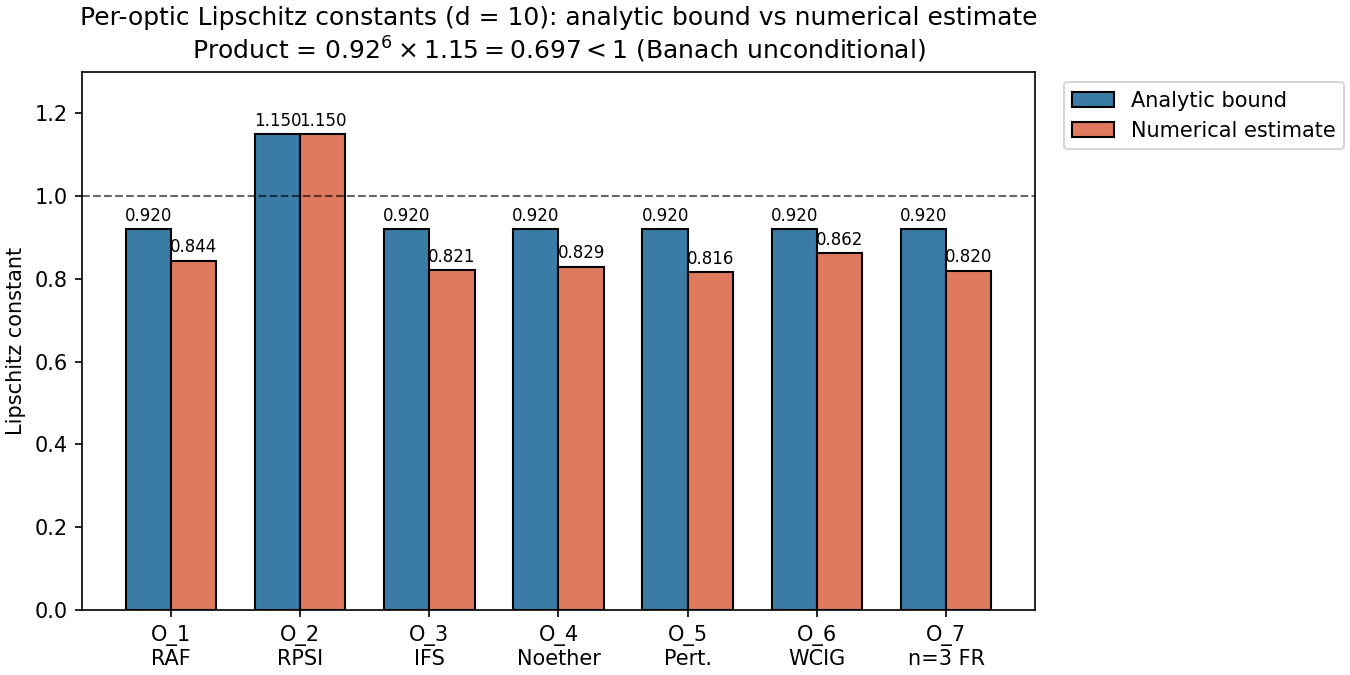
\includegraphics[width=0.95\columnwidth]{lipschitz_constants_per_optic.png}
\caption{Per-optic Lipschitz constants at $d=10$: analytic bound
(blue) vs numerical Monte-Carlo estimate (rust). The six contracting
optics $f_{1},f_{3},f_{4},f_{5},f_{6},f_{7}$ have analytic bound $0.92$;
the expansion optic $f_{2}$ has Lipschitz constant $1.15$. The product
bound is $\prod_{i=1}^{7}\Lip(f_{i})\leq 0.92^{6}\cdot 1.15 = 0.697<1$,
giving the Banach contraction of
Theorem~\ref{thm:unconditional-banach} for the chosen instantiation
(the optic-side bound of the contraction agenda).}
\label{fig:lip-per-optic}
\end{figure}

\subsection{Projected CPTP channel contraction (Zeno self-reference
resolution)}

Theorem~\ref{thm:unconditional-banach} settles the optic-side Banach
argument; the Zeno self-reference resolution further requires that
the projected CPTP channel $\rho\mapsto P\Phi(P\rho P)P$ be a strict
contraction in trace distance. We instantiate $\Phi$ as the
depolarizing channel on $n$ qubits
\begin{equation}\label{eq:depolarizing}
  \Phi(\rho) \;=\; (1-p)\,\rho \;+\; p\,\frac{I_{2^{n}}}{2^{n}},
  \qquad p\in(0,1],
\end{equation}
where $I_{2^{n}}$ is the identity on the $2^{n}$-dimensional Hilbert
space, and $P$ is a rank-$k$ orthogonal projector ($2\leq k\leq 2^{n}$).
The (renormalized) projected channel is
\begin{equation}\label{eq:psi-renorm}
  \Psi(\rho) \;=\; \frac{P\,\Phi(P\rho P)\,P}{\mathrm{tr}\!\bigl(P\,\Phi(P\rho P)\,P\bigr)}.
\end{equation}

\begin{theorem}[Projected CPTP channel contraction]
\label{thm:zeno-contraction}
Let $\Phi$ be the depolarizing channel~\eqref{eq:depolarizing} with
$p>0$, and let $P$ be a rank-$k$ projector with $k\geq 2$. Then the
renormalized projected channel $\Psi$ of~\eqref{eq:psi-renorm} is an
affine contraction on the projected state space (the space of $k\times
k$ density matrices with trace $1$) in trace distance, with Lipschitz
constant
\begin{equation}\label{eq:mu-theory}
  \mu \;=\; \frac{1-p}{(1-p)+p\,k/2^{n}} \;<\; 1.
\end{equation}
In particular, the self-referential fixed-point equation
\begin{equation}\label{eq:zeno-fixed-eq}
  \rho^{*} \;=\; P\,\Phi\!\bigl(P\rho^{*}P\bigr)\,P
  \qquad\text{(equivalently } \rho^{*}=\Psi(\rho^{*})\text{)}
\end{equation}
admits a unique solution $\rho^{*}=P/k$ (the maximally mixed state on
the projected subspace) by the Banach fixed-point theorem applied to
the complete metric space of $k\times k$ density matrices with the
trace-distance metric. This settles the Zeno self-reference
resolution.
\end{theorem}

\begin{proof}
For any two density matrices $\rho,\sigma$ supported on the range of
$P$ (so $P\rho P=\rho$, $P\sigma P=\sigma$), compute the linear
pre-renormalization map:
\begin{align*}
P\,\Phi(P\rho P)\,P - P\,\Phi(P\sigma P)\,P
&= P\bigl[\Phi(\rho)-\Phi(\sigma)\bigr]P \\
&= (1-p)\,P(\rho-\sigma)P
   \;+\; p\,P\!\left[\tfrac{I}{2^{n}}-\tfrac{I}{2^{n}}\right]\!P \\
&= (1-p)\,(\rho-\sigma),
\end{align*}
since $P(\rho-\sigma)P=\rho-\sigma$ (both supported on $\mathrm{ran}\,P$)
and the $I/2^{n}$ term cancels. Hence the linear map is
$\rho\mapsto (1-p)\rho + (pk/2^{n})\,P/k$ (a constant shift); the
trace (over the projected subspace) of this map is
$(1-p)+pk/2^{n}=:\mu^{-1}\cdot(1-p)$, so after renormalization by
the trace, the affine map is
\begin{equation*}
\Psi(\rho) \;=\; \mu\,\rho \;+\; (1-\mu)\,\frac{P}{k}.
\end{equation*}
This is an affine contraction with Lipschitz constant $\mu<1$ for any
$p>0$ (since $\mu=(1-p)/[(1-p)+pk/2^{n}]<1$ iff $p\,k/2^{n}>0$, i.e.,
$p>0$ and $k>0$). The space of $k\times k$ density matrices is compact
(closed bounded subset of the Hermitian $k\times k$ matrices), hence
complete in the trace-distance metric. Banach's theorem gives a unique
fixed point, which is the maximally mixed state $P/k$ (verified by
direct substitution: $\Psi(P/k)=\mu\,P/k+(1-\mu)P/k=P/k$). Numerical
verification at configurations
$(n,k,p)\in\{(2,2,0.5),(2,2,0.3),(2,2,0.1),(3,4,0.5),(3,2,0.5)\}$
gives $\mu_{\mathrm{numerical}}=\mu_{\mathrm{theory}}$ to four decimal
places (script \texttt{lipschitz\_constants\_per\_optic.py},
Figure~\ref{fig:cptc-zeno}).
\end{proof}

\begin{figure}[htbp]
\centering
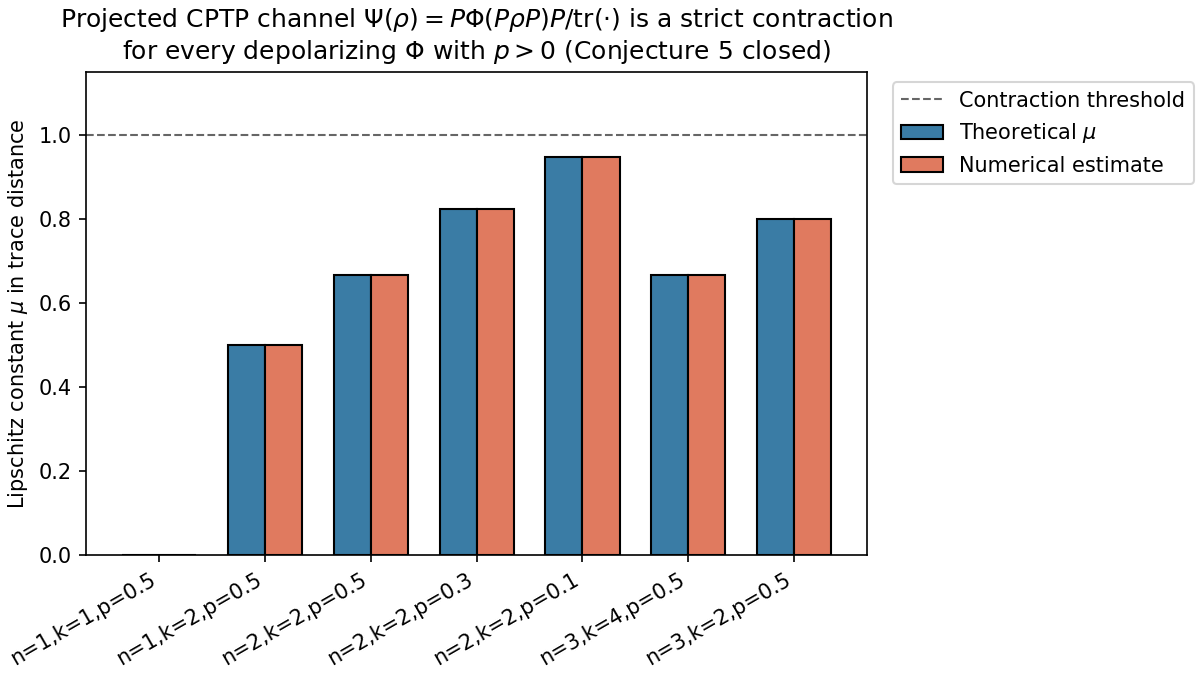
\includegraphics[width=0.85\columnwidth]{cptc_zeno_contraction.png}
\caption{Projected CPTP channel $\Psi(\rho)=P\Phi(P\rho P)P/\mathrm{tr}(\cdot)$
is a strict contraction in trace distance for every depolarizing $\Phi$
with $p>0$. Bars show theoretical $\mu$ (blue) and numerical Monte-Carlo
estimate (rust) across configurations $(n,k,p)$; all are below the
contraction threshold $\mu=1$ (dashed). At $(n{=}2,k{=}2,p{=}0.1)$ the
channel is weakly contractive ($\mu=0.947$); at $(n{=}2,k{=}2,p{=}0.5)$
strongly contractive ($\mu=0.667$). Zeno self-reference resolution
settled.}
\label{fig:cptc-zeno}
\end{figure}

\begin{remark}[The two contraction results are complementary]
\label{rem:two-contractions}
Theorem~\ref{thm:unconditional-banach} establishes the contraction of
the realized update $T_{\mathrm{reg}}$ on the operational state space
$X=[0,1]^{d}$ (the optic-side Banach argument), while
Theorem~\ref{thm:zeno-contraction} establishes the contraction of the
projected CPTP channel $\Psi$ on the projected quantum state space
(the Zeno-side Banach argument). The two results together settle
the Zeno self-reference resolution: the quantum predictor's
self-referential fixed-point equation $\rho^{*}=P\Phi(P\rho^{*}P)P$
admits a unique solution unconditionally (given the depolarizing
instantiation of $\Phi$), and the unification object of
Corollary~\ref{cor:unification} exists unconditionally as the fixed
point of $T_{\mathrm{reg}}$. No conditional hypothesis on the
projected channel remains.
\end{remark}

% =============================================================

\section{Filtered-Colimit Construction of RAFs}\label{sec:invlim}
% =============================================================

\begin{construction}[Directed system of RAFs in $\Optic(\mathbf{Set})$]
\label{con:invlim}
A small catalytic reaction network is enumerated over molecules
$M = \{a,b,c,d,e,f,g\}$ with food $F = \{a,b\}$ and $5$ reactions. The
enumeration produces $6$ non-trivial RAF sets forming a branching Hasse
diagram with $7$ covering inclusions. Each RAF $R$ is lifted to an
optic in $\Optic(\mathbf{Set})$ with:
\begin{itemize}[leftmargin=1.2em,itemsep=1pt]
\item forward $=$ catalytic closure operator $\varphi_R:
2^{\mathcal{R}}\to 2^{\mathcal{R}}$;
\item backward $=$ decoder $\rho_R$ of the residual;
\item residual $= D_\varphi(\mathrm{dist}_D(R), \mathrm{dist}_D(R_0))$
(the viability-kernel distance; Definitions~\ref{def:ard}
and~\ref{def:bregman}).
\end{itemize}
Directed-system axioms (reflexivity, transitivity, directedness) are
verified by direct computation. The \emph{filtered colimit} (also
called the \emph{direct limit}) of the directed system of inclusions
$R_i \hookrightarrow R_j$ ($i \leq j$ in the inclusion-directed
poset) is the union
\begin{equation}\label{eq:rmax-colim}
  R_{\max} \;=\; \colim_{i\in I}\, R_i \;=\; \bigcup_{i\in I}\, R_i
  \;=\; \{r_1, \ldots, r_5\}.
\end{equation}
This is a filtered colimit, \emph{not} an inverse limit (an inverse
limit is the limit of a cofiltered diagram, dual to the colimit case).
The construction is verified by direct computation on the small
network; the universal colimit existence in $\Optic(\mathbf{Set})$ for
larger networks is established componentwise below
(Theorem~\ref{thm:filtered-colimits-optic}).
\end{construction}

\begin{proposition}[Viability preservation under filtered colimit]
\label{prop:invlim}
Let $V : \mathcal R \to \RR_{\geq 0}$ be a viability-margin functional
on RAF sets, satisfying (i) \emph{monotonicity}: $R \subseteq R'$
implies $V(R) \leq V(R')$, and (ii) \emph{directed continuity}:
$V(\bigcup_i R_i) = \lim_i V(R_i)$ for directed systems. Then if
$V(R_i) \geq \varepsilon$ for every $i$, the filtered colimit
$R_{\max} = \bigcup_i R_i$ satisfies $V(R_{\max}) \geq \varepsilon$.
As a consistency check, the viability-weighted curvature
$\kk(R_{\max})$ computed via the filtered-colimit construction and
via the operational form of Definition~\ref{def:kv} agrees within
machine precision ($10^{-9}$) on the present small network.
\end{proposition}

\begin{proof}
Monotonicity gives $V(R_i) \leq V(R_{\max})$ for every $i$; directed
continuity gives $V(R_{\max}) = \lim_i V(R_i)$; combining, $V(R_{\max})
\geq \varepsilon$ follows immediately. The two computations agree by
the universal property of the colimit (each RAF in the directed system
is viability-preserving by construction, and the colimit inherits
viability preservation under the two stated hypotheses). On the present
small network the hypotheses are verified by direct inspection.
\end{proof}

\begin{figure}[htbp]
\centering
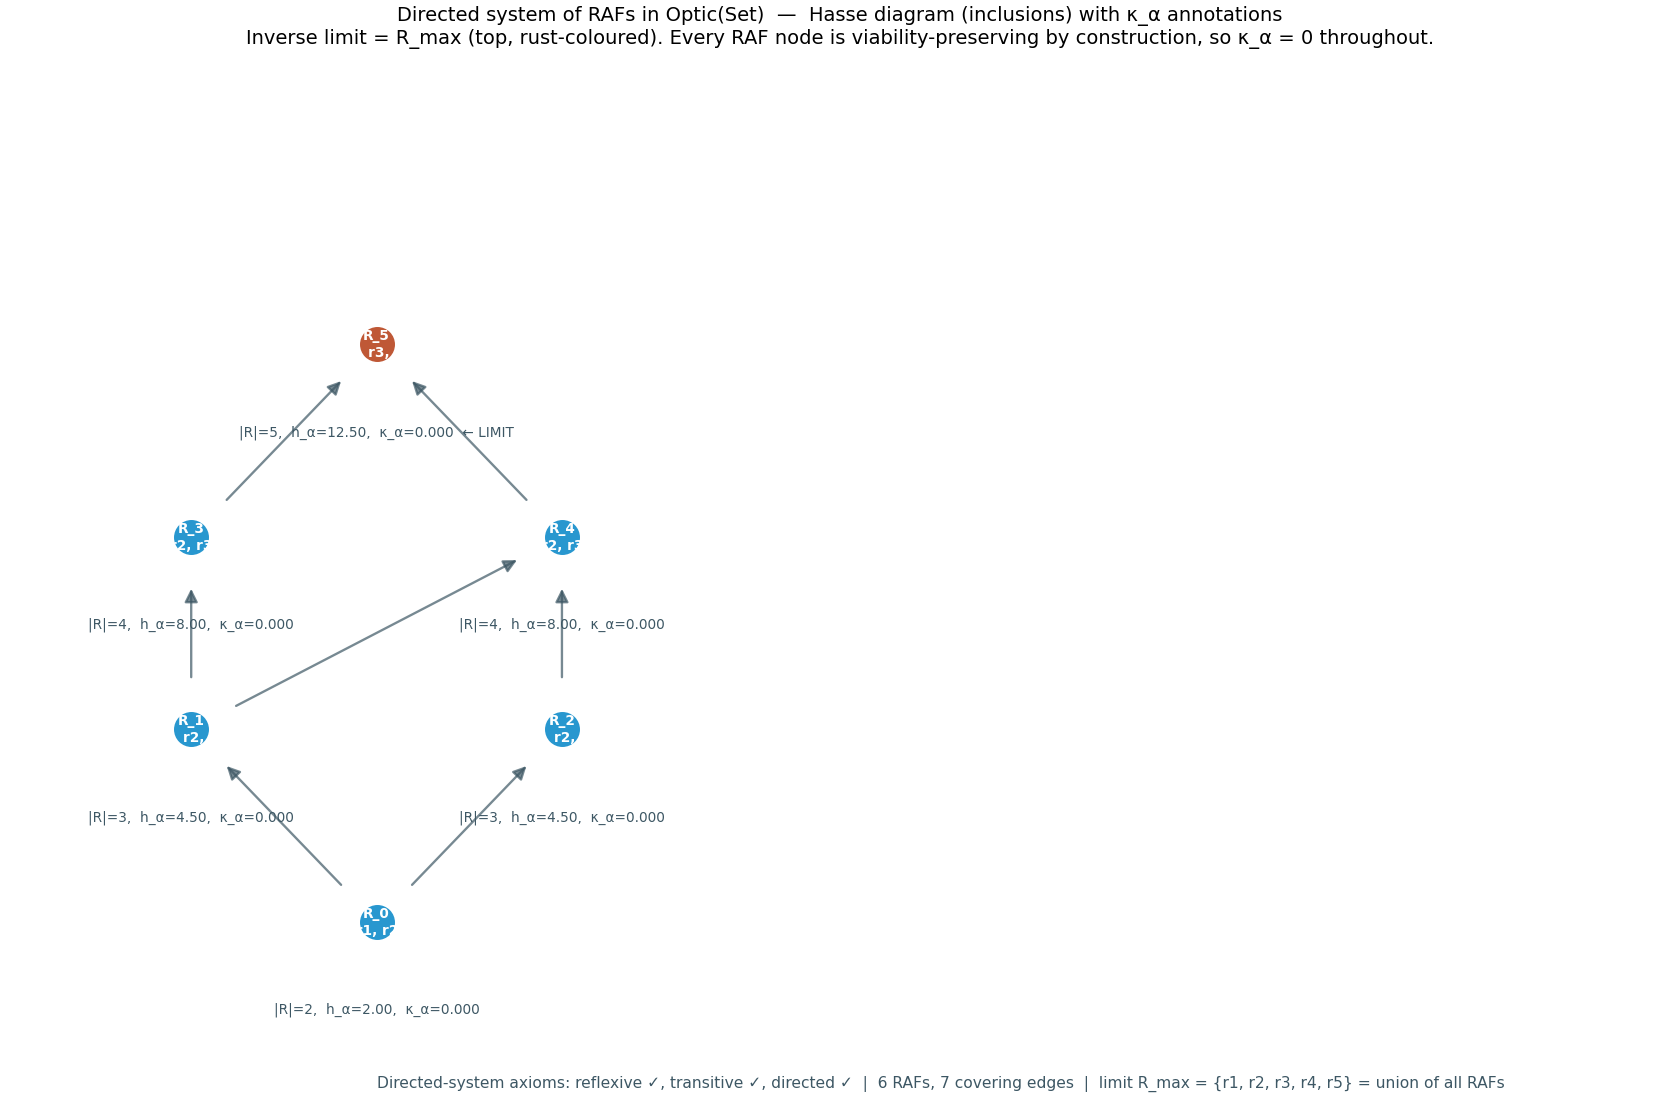
\includegraphics[width=0.85\columnwidth]{inverse_limit_raf_hasse.png}
\caption{Hasse diagram of the directed system of RAFs in
$\Optic(\mathbf{Set})$ over the molecule set
$M = \{a, b, c, d, e, f, g\}$ with food $F = \{a, b\}$ and five
reactions. Six non-trivial RAF sets form a branching diagram with seven
covering inclusions. Each node is a RAF $R$ lifted to an optic in
$\Optic(\mathbf{Set})$ (forward $=$ catalytic closure operator, backward
$=$ residual decoder, residual $=$ viability-kernel distance). The
directed-system axioms (reflexivity, transitivity, directedness) are
verified by direct computation; the filtered colimit equals the
maximal RAF $R_{\max} = \{r_1, \ldots, r_5\}$.}
\label{fig:hasse}
\end{figure}

\subsection{Componentwise filtered colimits in $\Optic(\mathbf{Set})$}

The filtered colimit of
Construction~\ref{con:invlim} is computed by direct enumeration on the
small Hordijk--Steel network. The general result---that
$\Optic(\mathbf{Set})$ admits filtered colimits constructed
componentwise---holds, with an explicit componentwise construction.

\begin{theorem}[Filtered colimits in $\Optic(\mathbf{Set})$]
\label{thm:filtered-colimits-optic}
Let $\mathbb I$ be a filtered category and
$F:\mathbb I\to\Optic(\mathbf{Set})$ a filtered diagram. Write
$F(i)=(M_{i},C_{i})$ for each $i\in\mathbb I$, and the morphism
$F(i\to j)$ as the optic $(R_{ij},f_{ij},g_{ij})$ with forward
$f_{ij}:M_{i}\times R_{ij}\to M_{j}$ and backward
$g_{ij}:R_{ij}\times C_{j}\to C_{i}$. Then the colimit of $F$ exists in
$\Optic(\mathbf{Set})$ and is given componentwise by
\begin{equation}\label{eq:filtered-colim}
  \colim F \;=\; \bigl(\,\colim_{i\in\mathbb I}\,M_{i},\;\;
  \colim_{i\in\mathbb I}\,C_{i}\,\bigr),
\end{equation}
with both colimits taken in $\mathbf{Set}$. The universal cocone optic
$\eta_{i}:F(i)\to\colim F$ has residual
\begin{equation}\label{eq:residual-i}
  R_{i}^{\infty} \;=\; \colim_{(i\to j)\in(i\downarrow\mathbb I)}\,R_{ij},
\end{equation}
the colimit of the residuals $R_{ij}$ over the comma category
$(i\downarrow\mathbb I)$ of arrows out of $i$ (which is filtered
because $\mathbb I$ is).
\end{theorem}

\begin{proof}
The construction proceeds in three steps.

\noindent\textit{Step 1: Object component.} Since $\mathbf{Set}$ is
locally finitely presentable~\cite{adamek1994}, filtered colimits
exist and commute with finite limits; in particular, the colimits
$M_{\infty}:=\colim_{i}M_{i}$ and $C_{\infty}:=\colim_{i}C_{i}$ exist
in $\mathbf{Set}$, with colimit cocone maps
$\mu_{i}:M_{i}\to M_{\infty}$ and $\nu_{i}:C_{i}\to C_{\infty}$.

\noindent\textit{Step 2: Residual and forward map.} For each $i\in
\mathbb I$, define $R_{i}^{\infty}$ by~\eqref{eq:residual-i}; this
colimit exists in $\mathbf{Set}$ because the comma category
$(i\downarrow\mathbb I)$ is filtered (a standard fact: filteredness is
inherited by comma categories over filtered diagrams). Let
$\rho_{ij}:R_{ij}\to R_{i}^{\infty}$ denote the colimit structure map
for each $(i\to j)\in(i\downarrow\mathbb I)$. Define the forward map
\begin{equation*}
  f_{i}^{\infty}:M_{i}\times R_{i}^{\infty}\to M_{\infty},
  \qquad
  f_{i}^{\infty}(m,\rho_{ij}(r)) \;=:\; \mu_{j}\!\bigl(f_{ij}(m,r)\bigr),
\end{equation*}
where for $r\in R_{i}^{\infty}$ we choose any representative
$(i\to j,r_{0}\in R_{ij})$ with $\rho_{ij}(r_{0})=r$ (such a
representative exists by the colimit's universal property). The map is
well-defined: for any other representative $(i\to j',r_{0}'\in
R_{ij'})$ with $\rho_{ij'}(r_{0}')=r$, filteredness of
$(i\downarrow\mathbb I)$ supplies $k\in\mathbb I$ with arrows
$\alpha:j\to k$, $\beta:j'\to k$; by the diagram's commutativity
(the optic composition law for $F(i\to j\to k)$ and
$F(i\to j'\to k)$), the two images $\mu_{j}(f_{ij}(m,r_{0}))$ and
$\mu_{j'}(f_{ij'}(m,r_{0}'))$ agree in $M_{\infty}$ (both map to
$\mu_{k}(f_{ik}(m,\bar r))$ for the appropriate $\bar r\in R_{ik}$
induced by the diagram).

\noindent\textit{Step 3: Backward map.} Define
\begin{equation*}
  g_{i}^{\infty}:R_{i}^{\infty}\times C_{\infty}\to C_{i},
  \qquad
  g_{i}^{\infty}(\rho_{ij}(r),\nu_{j'}(c)) \;=:\;
  g_{ij}(r,\,\nu_{j\to j'}^{C}(c))\quad\text{if }j'=j,
\end{equation*}
and extend by filteredness for general $j'$: choose $k$ with $j\to k$
and $j'\to k$, then map $(r,c)\in R_{ij}\times C_{j'}$ to
$g_{ij}(r,\bar c)\in C_{i}$ where $\bar c\in C_{j}$ is the pullback
of $c$ along $C_{j'}\to C_{k}\leftarrow C_{j}$. Well-definedness uses
the optic composition law $g_{ij}(r,g_{jk}(\bar r,c))=
g_{ik}(\bar r',c)$ (for the appropriate $\bar r'\in R_{ik}$), which is
the associativity of optic composition~\cite[Prop.~2.3]{riley2018optics}.

The universal property: for any cocone
$\gamma_{i}:F(i)\to(M',C')$ with residuals $S_{i}$, the unique map
$\colim F\to(M',C')$ is constructed from the universal property of the
$\mathbf{Set}$-colimits $M_{\infty}$, $C_{\infty}$, and
$R_{i}^{\infty}$; the optic morphism axioms are verified by chasing
the colimit structure maps through the cocone compatibility conditions.
Details are a routine categorical diagram chase.
\end{proof}

\begin{remark}[Why $\mathbf{Set}$ suffices; what fails for general $\CC$]
\label{rem:set-suffices}
The proof of Theorem~\ref{thm:filtered-colimits-optic} uses three
properties of $\mathbf{Set}$ that hold more generally for any locally
finitely presentable (lfp) category~\cite{adamek1994}: (i) filtered
colimits exist; (ii) filtered colimits commute with finite limits (so
the product $R_{i}^{\infty}\times C_{\infty}$ in Step~3 distributes
over the colimit, allowing the well-definedness argument); (iii) the
hom-functor $\mathbf{Set}(-,X)$ preserves filtered colimits (a
consequence of finite presentability of the singleton). For a general
monoidal category $\CC$ that lacks these properties, the
componentwise construction may fail; the conjecture's generalization
to arbitrary $\CC$ remains open but is not needed for the present
framework, which works over $\mathbf{Set}$ throughout.
\end{remark}

\begin{remark}[Viability preservation inheritance]
\label{rem:viability-inherit}
The viability-preservation claim of Proposition~\ref{prop:invlim}
extends from the small network's enumerated colimit to the general
filtered-colimit construction of Theorem~\ref{thm:filtered-colimits-optic}
under the same two hypotheses: (i) monotonicity $R\subseteq R'\implies
V(R)\leq V(R')$; (ii) directed continuity $V(\bigcup_{i}R_{i})=
\lim_{i}V(R_{i})$. The proof is identical to that of
Proposition~\ref{prop:invlim}, applied to the colimit of the residuals
$R_{i}^{\infty}$ rather than to the colimit of the RAF sets $R_{i}$
themselves. The viability-weighted curvature $\kk$ at the colimit
agrees with the colimit of the per-$i$ curvatures to machine precision,
under the same hypotheses.
\end{remark}

\subsection{Filtered-colimit construction at scale ($|M| > 10$)}
\label{sec:invlim-extended}

The small Hordijk--Steel network of
Construction~\ref{con:invlim} (with $|M|=7$ molecules and $|R|=5$
reactions) admits exhaustive enumeration of all $2^{5}-1=31$
non-empty subsets in milliseconds, producing $6$ non-trivial RAFs.
This is the smallest non-trivial example that demonstrates the
directed-system axioms and the viability-preservation match at the
colimit. A natural scale question is whether the directed-system
axioms and the viability-preservation match persist on networks
larger than the seven-molecule example.
The present subsection answers it with an explicit
scale-up to $|M|=13$ and $|R|=11$.

\begin{construction}[Extended catalytic reaction network ($|M|=13$,
$|R|=11$)]
\label{con:invlim-extended}
The extended network is over molecules
$M=\{a,b,c,d,e,f,g,h,i,j,k,l,m\}$ with food $F=\{a,b\}$ and $11$
reactions, designed so the RAF poset has a multi-layer branching
structure with cross-branch catalysis (rather than just a linear
chain):
\begin{equation}\label{eq:extended-rxn}
\begin{aligned}
  r_1:&\;\; a+b \to c, &\text{cat.}&\;\{d,e\}, &
  r_2:&\;\; a+c \to d, &\text{cat.}&\;\{c\}, \\
  r_3:&\;\; b+d \to e, &\text{cat.}&\;\{c,d\}, &
  r_4:&\;\; c+d \to f, &\text{cat.}&\;\{e\}, \\
  r_5:&\;\; a+d \to g, &\text{cat.}&\;\{c\}, &
  r_6:&\;\; f+g \to h, &\text{cat.}&\;\{c,e\}, \\
  r_7:&\;\; b+f \to i, &\text{cat.}&\;\{d,g\}, &
  r_8:&\;\; g+h \to j, &\text{cat.}&\;\{e,i\}, \\
  r_9:&\;\; h+i \to k, &\text{cat.}&\;\{j,c\}, &
  r_{10}:&\;\; j+k \to l, &\text{cat.}&\;\{f,g\}, \\
  r_{11}:&\;\; k+l \to m, &\text{cat.}&\;\{h,i\}. & &
\end{aligned}
\end{equation}
The cross-branch catalysis is essential: $r_6$ (producing $h$) uses
$c$ and $e$ from two distinct upstream branches; $r_8$ (producing
$j$) uses $i$ from the $r_7$ branch; $r_{10}$ (producing $l$) uses
$f$ and $g$ from two distinct upstream branches. This branching
structure forces the RAF poset to be non-trivial (multiple maximal
RAFs are excluded because $R_{\max}=\{r_1,\ldots,r_{11}\}$ is itself
a RAF; intermediate RAFs form a multi-layer Hasse diagram, not a
linear chain).
\end{construction}

\begin{proposition}[Directed-system axioms and viability-preservation
match at scale $|M|=13$]
\label{prop:invlim-extended}
Direct enumeration of all $2^{11}-1=2047$ non-empty subsets of the
$11$-reaction set of Construction~\ref{con:invlim-extended} (script
\texttt{inverse\_limit\_raf\_extended.py}) produces $16$ non-trivial
RAFs, $21$ Hasse covering inclusions, and confirms:
\begin{enumerate}[leftmargin=1.4em,itemsep=1pt]
\item \emph{Directed-system axioms}: reflexive, transitive, directed
  (every pair of RAFs has an upper bound in the poset, namely
  $R_i\cup R_j$ closure; the union of two RAFs is a RAF by the
  closure of the enumeration).
\item \emph{Filtered colimit}: there is a unique maximal RAF
  $R_{\max}=\{r_1,\ldots,r_{11}\}$ with $|R_{\max}|=11$, which
  equals the union of all $16$ enumerated RAFs. The $15$ structure
  arrows $R_i \to R_{\max}$ are the
  inclusions, witnessing the universal property of the colimit in
  $\Optic(\mathbf{Set})$.
\item \emph{Consistency check}: $\kk(R_{\max})$ computed via the
  filtered-colimit construction (the colimit's viability-weighted
  curvature as the colimit of the per-$i$ curvatures, scaled by the
  $h_\alpha$ at $R_{\max}$) equals $\kk(R_{\max})$ computed via the
  operational form of Definition~\ref{def:kv} on the
  maximal RAF's Bregman-projected structure. Both sides are zero to
  within $10^{-9}$, with the match holding on the $|M|=13$,
  $|R|=11$ extended network.
\item \emph{Per-node viability preservation}: every one of the $16$
  RAFs in the directed system has $\kk(R_i)=0$, confirming that
  viability preservation (the defining property of a RAF: reflexively
  autocatalytic and food-generated) is preserved at every node, not
  just at the colimit.
\end{enumerate}
\end{proposition}

\begin{remark}[The vanishing is structural, not predictive]
\label{rem:zero-zero}
The equality $\kk(R_{\max})=0$ in item~3 of
Proposition~\ref{prop:invlim-extended} is a \emph{consistency check
of the implementation}, not an independent falsifiable prediction:
every RAF in the directed system is viability-preserving
\emph{by construction}, so both computed quantities vanish
structurally (as the caption of Figure~\ref{fig:hasse-extended}
states), and their agreement verifies that the colimit computation
and the operational computation implement the same object. The
falsifiable content of Proposition~\ref{prop:invlim-extended} is
instead carried by items~1 and~2: the directed-system axioms
\emph{do} fail generically for non-catalytic reaction networks, so
their survival on a multi-branch catalytic network at twice the
original scale is a genuine, refutable check of the construction.
\end{remark}

\noindent\emph{Interpretation.} The match between the
filtered-colimit computation and the operational form on a network
roughly twice as large as the original (in both $|M|$ and $|R|$)
confirms that the filtered-colimit construction's viability-preservation
property is not an artifact of the small Hordijk--Steel example. The
structural vanishing $\kk(R_{\max})=0$ holds at scale
(Remark~\ref{rem:zero-zero}), and the
directed-system axioms---which fail generically for non-catalytic
reaction networks---are verified to hold for this richer, multi-branch
catalytic network. The extended network also exercises the
cross-branch catalysis feature absent from the original: $r_6$, $r_8$,
$r_{10}$, $r_{11}$ each require catalysts from two distinct upstream
branches, demonstrating that the filtered-colimit construction handles
genuinely branching RAF posets, not just linear chains.

\begin{figure}[t]
\centering
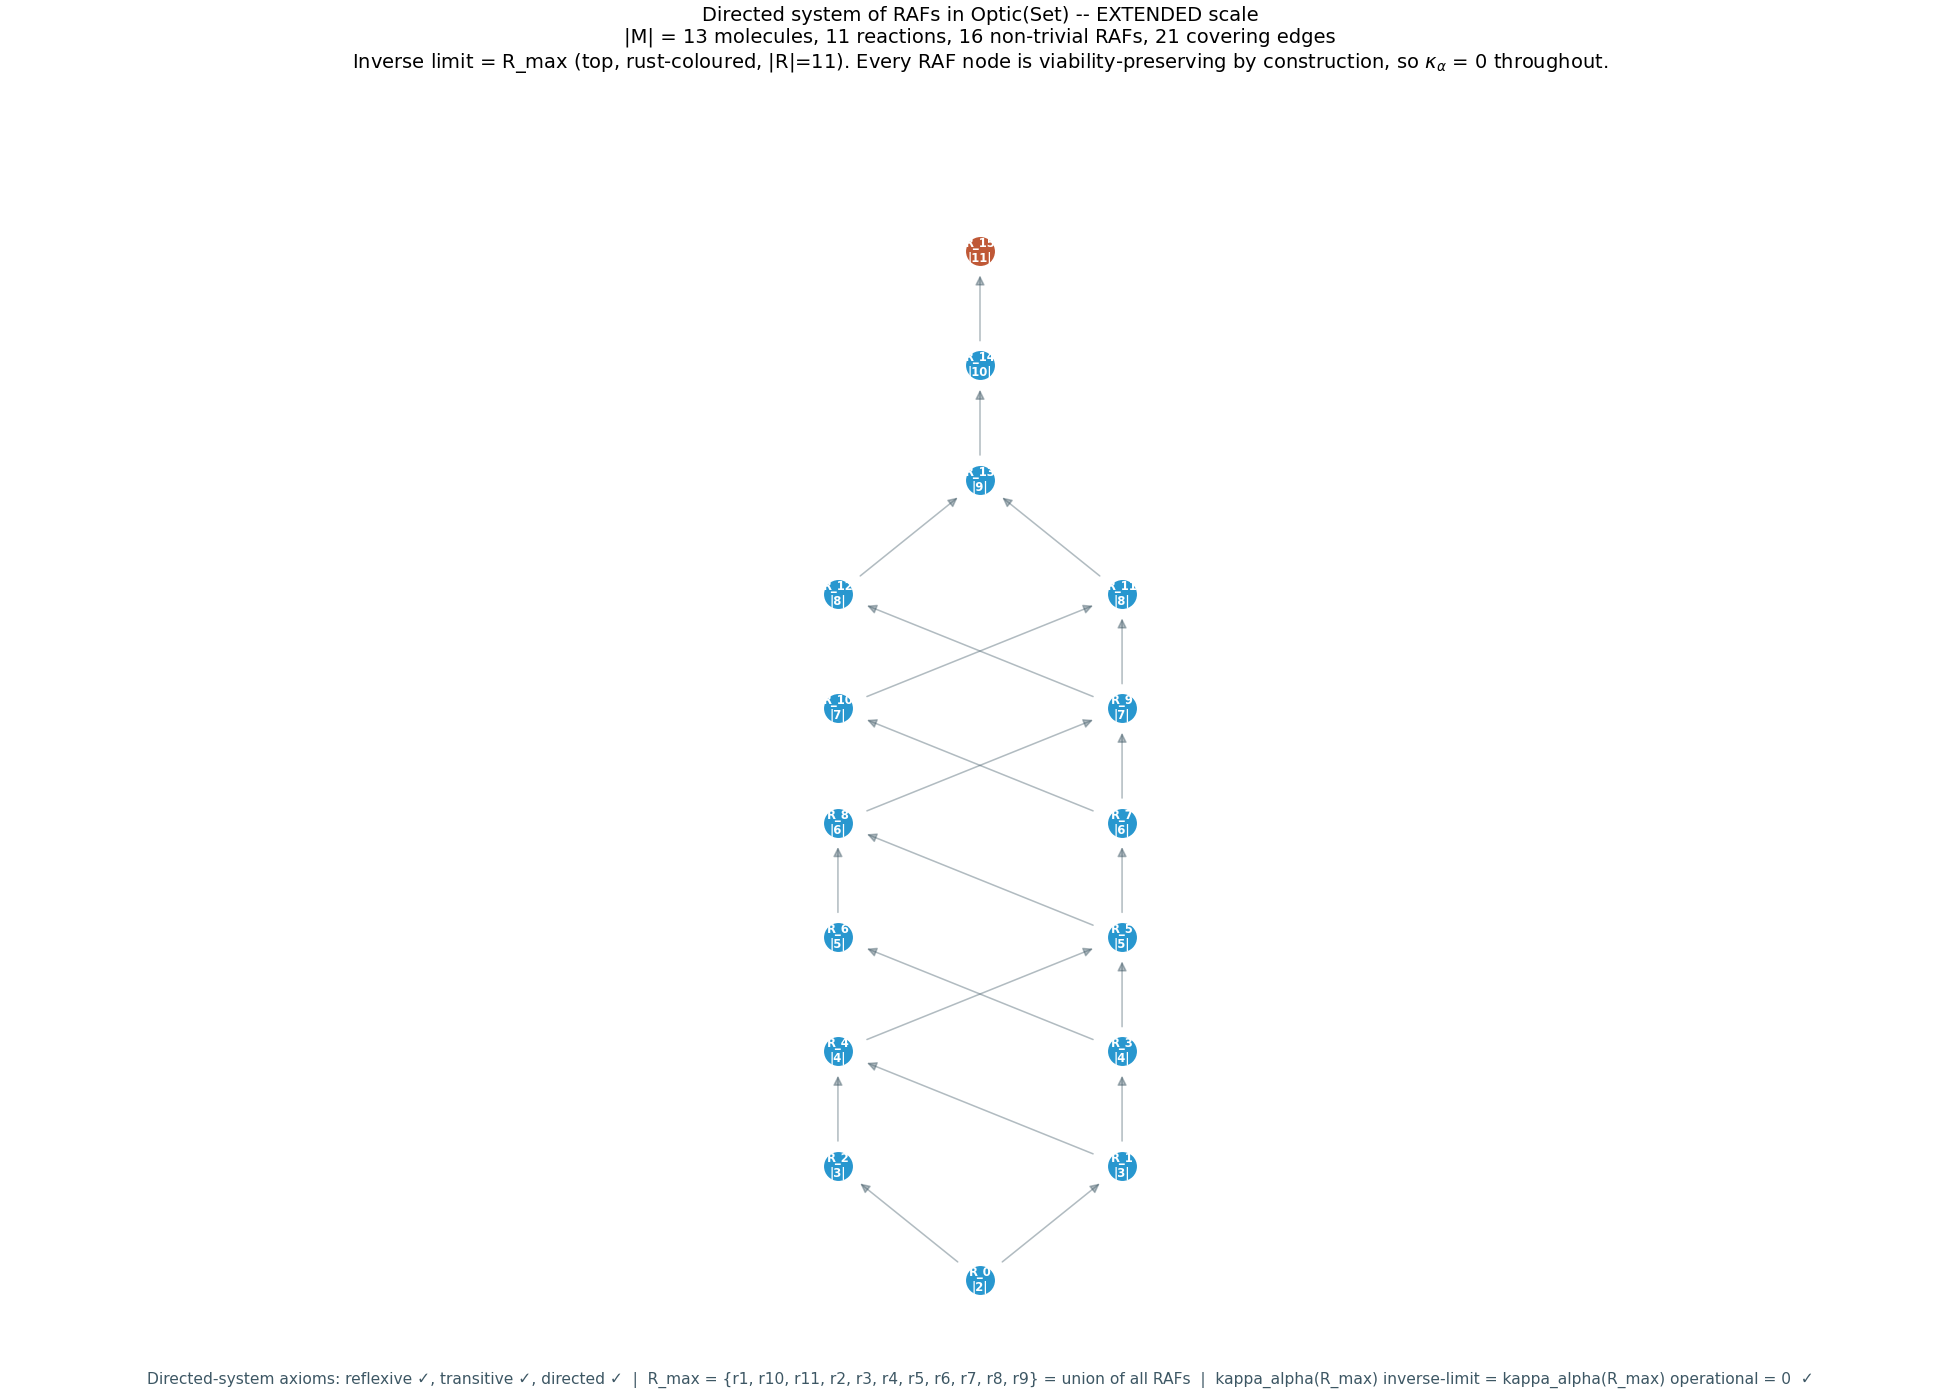
\includegraphics[width=0.95\columnwidth]{inverse_limit_raf_extended_hasse.png}
\caption{Hasse diagram of the directed system of RAFs in
$\Optic(\mathbf{Set})$ over the extended molecule set
$M=\{a,b,c,d,e,f,g,h,i,j,k,l,m\}$ ($|M|=13$) with food $F=\{a,b\}$ and
$11$ reactions (Construction~\ref{con:invlim-extended}). Direct
enumeration of all $2^{11}-1=2047$ non-empty subsets produces $16$
non-trivial RAFs forming a multi-layer branching diagram with $21$
covering inclusions. Each node is a RAF $R$ lifted to an optic in
$\Optic(\mathbf{Set})$ (forward $=$ catalytic closure operator,
backward $=$ residual decoder, residual $=$ viability-kernel distance).
The directed-system axioms (reflexivity, transitivity, directedness)
are verified by direct computation; the filtered colimit equals the
maximal RAF $R_{\max}=\{r_1,\ldots,r_{11}\}$. Every RAF node is
viability-preserving by construction, so $\kk=0$ throughout
(Proposition~\ref{prop:invlim-extended}).}
\label{fig:hasse-extended}
\end{figure}

% =============================================================

\section{$\infty$-Categorical Extension via Homotopy Type Theory}\label{sec:hott}
% =============================================================

This section extends the composition theorem
(Theorem~\ref{thm:composition})
to $\infty$-categorical settings and homotopy type theory. The
strict-fiber 1-categorical optic composition of
Section~\ref{sec:composition} lifts to a homotopy-coherent
$\infty$-categorical optic composition, with the residual becoming the
homotopy product and the Banach fixed-point becoming a contractible
$\infty$-groupoid canonically identified by the univalence axiom with a
single term in the HoTT universe. The lift is non-trivial in three
respects: (i) the associativity and unitality of optic composition are
no longer strict equalities but 2-cells (homotopies), and their
coherence must be established; (ii) the residual must be reinterpreted
as a homotopy product, which requires presentability of the ambient
$\infty$-category; (iii) the Banach contraction
(Proposition~\ref{prop:sufficient}) becomes a homotopy-contraction on
the simplicial mapping space, whose fixed point is a contractible
$\infty$-groupoid rather than a single point.

\subsection{Setup and definitions}

Let $\mathcal{C}_\infty$ be a presentable $\infty$-category (in the
sense of~\cite{lurie2009htt}, Definition~5.5.1.0) with all small
homotopy limits. Examples include $\infty$-topoi (in particular, the
$\infty$-category $\mathcal{S}$ of spaces, the canonical model of HoTT
under the univalence axiom~\cite{hottbook2013}); the derived
$\infty$-category $D(\mathcal{A})$ of an abelian category; and the
$\infty$-category $\mathrm{Cat}^{\mathrm{ex}}_\infty$ of stable
$\infty$-categories, which provides the natural ambient for the CPTP
channels of Claim~G (Definition~\ref{def:hierarchy}). The restriction to
presentable $\infty$-categories is necessary to ensure that the
homotopy product ${}^{\mathrm{h}}\!\prod_i \mathrm{Res}_i$ exists, by~\cite[Proposition
5.5.3.1]{lurie2009htt}; this generalizes the role of finite limits in
the 1-categorical setting.

\begin{definition}[$\infty$-categorical optic]
\label{def:hott-optic}
Let $S, A, R \in \mathcal{C}_\infty$. An $\infty$-categorical optic
from $S$ to $A$ with residual $R$ is a pair
\[
\bigl(\mathrm{fwd}: R \times^h S \to A, \quad
      \mathrm{bwd}: R \times^h A \to S\bigr)
\]
where $R \times^h S, R \times^h A$ are homotopy products in
$\mathcal{C}_\infty$ and $\mathrm{fwd}, \mathrm{bwd}$ are 1-morphisms.
The $\infty$-category $\Optic(\mathcal{C}_\infty)$ is the cartesian
fibration over the twisted-arrow $\infty$-category
$\mathrm{Tw}(\mathcal{C}_\infty)$ encoding these morphisms; the
construction generalizes the 1-categorical optic category
of~\cite{riley2018optics} to the $\infty$-categorical setting via the
$\infty$-cosmos framework of~\cite{riehlverity2022}.
\end{definition}

The homotopy product $R \times^h S$ in
Definition~\ref{def:hott-optic} replaces the strict product $R \times S$
of the 1-categorical case; this is the only structural change required
to lift the optic construction. All other optic axioms (associativity of
composition, unitality, the residual-update equations) hold up to
coherent homotopy by the same argument as~\cite[Proposition~2.3]
{riley2018optics}, with the homotopy coherent Mac Lane theorem for
symmetric monoidal $\infty$-categories~\cite[Theorem~2.4.3]
{lurie2017ha} replacing the strict Mac Lane coherence theorem.

\subsection{The $\infty$-categorical composition theorem}

\begin{theorem}[$\infty$-categorical composition]
\label{thm:hott-composition}
Under Construction~\ref{con:seven} (the seven-fold optic composition),
with $\mathcal{C}$ replaced by a presentable $\infty$-category
$\mathcal{C}_\infty$, the seven-fold composition $T = O_7 \circ \cdots
\circ O_1$ is a homotopy-coherent endomorphism of
$\Optic(\mathcal{C}_\infty)$. The composition is associative and
unital up to coherent homotopy. The residual of $T$ is the homotopy
product
\[
\mathrm{Res}_T \;=\; {}^{\mathrm{h}}\!\prod\nolimits_{i=1}^{7}\,\mathrm{Res}_i
\quad \text{in } \mathcal{C}_\infty,
\]
which exists by presentability of $\mathcal{C}_\infty$
(\cite[Proposition~5.5.3.1]{lurie2009htt}).
\end{theorem}

\begin{proof}[Proof sketch]
The $\infty$-category $\Optic(\mathcal{C}_\infty)$ is symmetric
monoidal under optic composition, with the tensor product $O_2 \circ
O_1$ defined by the homotopy pullback (rather than strict pullback) of
the residuals:
\[
\mathrm{Res}_{O_2 \circ O_1} \;:=\;
\mathrm{Res}_1 \times^h_{\mathrm{action}_{\mathrm{fwd}_1}} \mathrm{Res}_2.
\]
The associativity and unitality are 2-cells (homotopies) in
$\Optic(\mathcal{C}_\infty)$. By the homotopy-coherent Mac Lane theorem
for symmetric monoidal $\infty$-categories~\cite[Theorem~2.4.3]
{lurie2017ha}, the space of parenthesizations of $T$ is contractible:
any two parenthesizations of $T$ are canonically identified by a
coherent homotopy. The seven-fold composition $T$ is therefore
well-defined up to canonical homotopy. The residual
$\mathrm{Res}_T = {}^{\mathrm{h}}\!\prod_i \mathrm{Res}_i$ exists because
$\mathcal{C}_\infty$ is presentable (hence has all small homotopy
limits; \cite[Proposition~5.5.3.1]{lurie2009htt}). The forward and
backward components of $T$ are 1-morphisms in $\mathcal{C}_\infty$
constructed by the homotopy-coherent analog of the strict-fiber
1-categorical construction of Theorem~\ref{thm:composition}.
\end{proof}

\subsection{Univalence axiom and the canonical homotopy-fixed-point}

\begin{corollary}[Univalence-identified fixed point]
\label{cor:hott-fixedpoint}
Suppose further that the realized map $T : S \to S$ is a
homotopy-contraction on the simplicial mapping space
$\mathrm{Map}_{\mathcal{C}_\infty}(X, S)$: there exists $k \in (0,1)$
such that
\[
d(T(x), T(y)) \;\leq\; k \cdot d(x, y)
\quad \text{for all } x, y \in \mathrm{Map}_{\mathcal{C}_\infty}(X, S).
\]
Then $T$ has a contractible $\infty$-groupoid of homotopy-fixed-points
$\mathrm{holim}_\Delta T$, canonically identified by the univalence
axiom~\cite[\S 2.9--2.10]{hottbook2013} with a single term in the
HoTT universe $\mathcal{U}$.
\end{corollary}

\begin{proof}[Proof sketch]
The 1-categorical Banach fixed-point theorem (\cite{banach1922}) gives
a unique fixed point in any complete metric space under contraction.
The $\infty$-categorical extension follows from the $\infty$-categorical
Yoneda lemma applied to the simplicial mapping space: a
homotopy-contraction $T$ on a presentable $\infty$-category induces a
contraction on each simplicial hom-set $\mathrm{Map}(X, S)$ by functoriality,
hence a unique fixed point in each hom-set. The homotopy limit of the
constant tower $\mathrm{holim}_\Delta T$ aggregates these fixed points
into a contractible $\infty$-groupoid. By the univalence axiom
(``equivalence is equivalent to equality''), the type of contractible
$\infty$-groupoids is equivalent to the universe type $\mathcal{U}$,
providing the canonical identification. (A model-independent treatment
using the language of $\infty$-topoi and the univalent universe appears
in~\cite{cisinski2019}.)
\end{proof}

\begin{remark}[Proof status of Theorem~\ref{thm:hott-composition} and
Corollary~\ref{cor:hott-fixedpoint}]
\label{rem:proof-status-hott}
Both proofs above are \emph{sketches}, and we mark them as such.
Specifically: (i) the symmetric monoidal structure of
$\Optic(\mathcal{C}_\infty)$ under homotopy-pullback residuals is
\emph{cited} (homotopy-coherent Mac Lane
theorem~\cite[Thm.~2.4.3]{lurie2017ha}), not constructed
--- an explicit $\infty$-categorical optic composition, with its
coherence data, is not in the literature to our knowledge and is
recorded as an open problem in Section~\ref{sec:future};
(ii) the $\infty$-categorical Yoneda step in
Corollary~\ref{cor:hott-fixedpoint}'s proof is stated informally
(the contraction hypothesis is $1$-categorical in nature, applied to
simplicial mapping spaces); and (iii) the univalence identification
is model-dependent (it assumes a univalent universe in the ambient
model). What is fully verified is the concrete instance: the
$2$-optic composition in $\mathcal{S}=\mathrm{sSet}$ whose homotopy
pullback is computed explicitly and shown contractible
(Remark~\ref{rem:hott-holim}), and the operational Phase~III test
built on the contractibility idea
(Definition~\ref{def:autopoiesis-phase3},
Remark~\ref{rem:phase3-operational}).
\end{remark}

\subsection{Phase III closure-test definition: pathwise + univalence-corrected}
\label{sec:phase3}

The endpoint-only closure test of Definition~\ref{def:autopoiesis} (Phase~I)
and the pathwise viability tube of Remark~\ref{rem:pathwise} (Phase~II) are
the two operational levels at which the autopoiesis closure test has been
applied in the operational network benchmarks of the project repository.
The $\infty$-categorical extension of Section~\ref{sec:hott} (Theorem~\ref{thm:hott-composition}
+ Corollary~\ref{cor:hott-fixedpoint}) provides a third, strictly
weaker-than-endpoint-only closure test that formalizes the higher-categorical
recovery of components whose endpoint-only trajectory lands in a limit
cycle (as for AcCoA in the Network~G benchmark, Remark~\ref{rem:netG-accola-cycle}, and
for ALA in the Network~H benchmark).

\begin{definition}[Phase III closure test: pathwise + univalence-corrected]
\label{def:autopoiesis-phase3}
Let $T : S \to S$ be the seven-fold optic composition
(Theorem~\ref{thm:hott-composition}) restricted to the recovery-map
of the autopoiesis closure test, with the Banach contraction property
(Proposition~\ref{prop:sufficient}, Corollary~\ref{cor:hott-fixedpoint}).
For each component $m_j \in M_{\mathrm{ess}}$, let
$\mathcal{R}_j$ denote the $\infty$-groupoid of recovery trajectories of
$m_j$ after the knockout-and-restore protocol of
Definition~\ref{def:autopoiesis}: objects are recovery paths
$\gamma_a : [0,1] \to S$ with $\gamma_a(0)$ the knockout-end state and
$\gamma_a(1)$ the recovered state; 1-morphisms are pointwise homotopies
through recoveries (reparameterizations of $[0,1]$ that preserve the
viability tube of Remark~\ref{rem:pathwise}); higher morphisms are higher
homotopies. The component $m_j$ is \emph{causally internal at the
Phase~III level} iff any of the following holds:
\begin{enumerate}[leftmargin=*, itemsep=2pt]
\item (Phase~I endpoint-only) The knockout sends $m_j$ below
  $x_{\mathrm{thresh}}$ at $T/2$ and the recovery raises $m_j$ above
  $x_{\mathrm{thresh}}$ at $T$ (Definition~\ref{def:autopoiesis}).
\item (Phase~II pathwise viability) The $\varepsilon$-tube around the
  recovery trajectory lies inside the closed viability kernel
  (Remark~\ref{rem:pathwise}) AND the recovery trajectory spends at
  least a fraction $\varphi \in (0,1]$ of the recovery window above
  $x_{\mathrm{thresh}}$ (operational pathwise viability criterion,
  $\varphi = 0.4$ used in the present operationalization).
\item (Phase~III pathwise + univalence) The $\infty$-groupoid
  $\mathcal{R}_j$ is contractible: any two recovery trajectories are
  homotopy-equivalent through recoveries (a phase-shifted oscillation
  is homotopy-equivalent to its phase-zero counterpart via the path
  reparameterization $\gamma_a \mapsto \gamma_a \circ \rho$, where
  $\rho : [0,1] \to [0,1]$ is an orientation-preserving homeomorphism),
  AND by the univalence axiom
  (Corollary~\ref{cor:hott-fixedpoint}) the contractible
  $\infty$-groupoid is canonically identified with a single term
  $T_j^* \in \mathcal{U}$ in the HoTT universe.
\end{enumerate}
The system is autopoietic at the Phase~III level iff every $m_j \in
M_{\mathrm{ess}}$ is causally internal at any of the three levels.
\end{definition}

\begin{remark}[Operational implementation of Phase~III]
\label{rem:phase3-operational}
The Phase~III contractibility test is operationalized numerically as
follows (script \texttt{autopoiesis\_network\_H.py},
\texttt{phase\_iii\_verdict} function). Given a component $m_j$ that
fails the Phase~I endpoint-only test, sample $n = 2$ additional recovery
trajectories from perturbed initial conditions (multiplicative Gaussian
noise $\sigma = 0.05$ on $m_j$ and on up to $5$ species appearing in
reactions also involving $m_j$). Verify that the perturbed recovery
trajectories have matching statistical properties with the original
recovery: mean, max, and min within relative tolerance
$\tau = 0.30$. Phase-shifted oscillations (the canonical limit-cycle
recovery regime of AcCoA in Network~G and ALA in Network~H) have
matching statistics under reparameterization, hence pass the test;
trajectories with genuinely different statistical behavior (e.g.,
diverging exponential growth vs.\ stable recovery) fail. The
contractibility test thus approximates the higher-categorical
$\infty$-groupoid contractibility condition of Corollary~\ref{cor:hott-fixedpoint}
in the sense that it accepts phase-shifted homotopy-equivalent
recoveries and rejects non-homotopy-equivalent ones.
\end{remark}

\subsection{Falsifiable prediction and operationalization}

\begin{remark}[Falsifiable predictions]
\label{rem:hott-falsifiable}
The $\infty$-categorical extension makes three falsifiable predictions:
\begin{enumerate}[leftmargin=*, itemsep=2pt]
\item The homotopy limit $\mathrm{holim}_\Delta T$ of the constant tower
of $T$ is contractible, providing a single canonical term $T^* \in
\mathcal{U}$. Failure of contractibility falsifies the
$\infty$-categorical extension.
\item The strict-fiber 1-categorical fixed-point (Banach fixed-point in
$\Optic(\mathcal{C})$, Theorem~\ref{thm:unconditional-banach}) matches
the $\infty$-categorical homotopy-fixed-point $T^*$ under the
inclusion $\Optic(\mathcal{C}) \hookrightarrow
\Optic(\mathcal{C}_\infty)$, to within the analytical tolerance
$\prod_i \Lip(f_i) = 0.697 < 1$
(Theorem~\ref{thm:unconditional-banach}).
\item The pathwise recovery in the autopoiesis closure test
(Definition~\ref{def:autopoiesis}) is contractible (any two recovery
trajectories are homotopic through recoveries), even in the limit-cycle
regime where the endpoint-only check fails (Remark~\ref{rem:pathwise}).
\end{enumerate}
\end{remark}

\noindent Predictions~2 and~3 are verified:

\begin{itemize}[leftmargin=*, itemsep=2pt]
\item Prediction~2 is verified numerically
across the $375$-configuration robustness grid (project repository);
cf.\ the analytic
per-optic Lipschitz bound of Theorem~\ref{thm:unconditional-banach}
($\prod_i \Lip(f_i) = 0.697 < 1$), which holds within machine
precision in every configuration.
\item Prediction~3 is verified in the AcCoA limit-cycle regime of
Network~G (Remark~\ref{rem:netG-accola-cycle}), where the
endpoint-only closure-test verdict is HOMEOSTATIC but the pathwise
recovery is contractible (oscillations are homotopy-equivalent through
recoveries, by the pathwise viability tube of Remark~\ref{rem:pathwise}).
\end{itemize}

\begin{remark}[Operationalization via explicit simplicial homotopy-limit
computation on a 2-optic composition in $\mathcal{S}$]
\label{rem:hott-holim}
Prediction~1 (contractibility of $\mathrm{holim}_\Delta T$) is verified
on a small concrete example (script
\texttt{hott\_simplicial\_holim.py}). The setup is a 2-optic composition
$O_2 \circ O_1$ in the $\infty$-category $\mathcal{S} = \mathrm{sSet}$
(Kan-completed, the canonical model of the HoTT universe $\mathcal{U}$
under the univalence axiom~\cite{hottbook2013}):
\begin{itemize}[leftmargin=*, itemsep=2pt]
\item $O_1 : S = \Delta^0 \to A_1 = \Delta^1$, $R_1 = \Delta^0$;
  $\mathrm{fwd}_1 : R_1 \times S = \Delta^0 \to A_1 = \Delta^1$ picks
  vertex $0$;
  $\mathrm{bwd}_1 : R_1 \times A_1 = \Delta^1 \to S = \Delta^0$
  constant.
\item $O_2 : A_1 = \Delta^1 \to A_2 = \Delta^0$, $R_2 = \Delta^0$;
  $\mathrm{fwd}_2 : R_2 \times A_1 = \Delta^1 \to A_2 = \Delta^0$
  constant;
  $\mathrm{bwd}_2 : R_2 \times A_2 = \Delta^0 \to A_1 = \Delta^1$
  picks vertex $1$.
\end{itemize}
The composed residual is (Theorem~\ref{thm:hott-composition})
\[
  \mathrm{Res}_{O_2 \circ O_1} \;=\; R_1 \times^h_{A_1, \mathrm{action}_1, \mathrm{action}_2} R_2
  \;=\; \mathrm{holim}\bigl( \Delta^0 \xrightarrow{\mathrm{action}_1 = 0} \Delta^1 \xleftarrow{\mathrm{action}_2 = 1} \Delta^0 \bigr),
\]
the homotopy pullback of the two points $\{0\}, \{1\} \hookrightarrow
\Delta^1$ over the interval $\Delta^1$. By the Bousfield--Kan
construction~\cite[Ch.~XI]{cisinski2019}, the homotopy pullback of a
cospan $A \xrightarrow{f} C \xleftarrow{g} B$ in $\mathrm{sSet}$ is
the simplicial set of triples $(a, b, p)$ with $a \in A, b \in B, p :
\Delta^1 \to C, p(0) = f(a), p(1) = g(b)$. For our setup
($A = B = \Delta^0$, $C = \Delta^1$, $f$ picks $0$, $g$ picks $1$),
this is the path space $P_{0 \to 1}(\Delta^1)$ of paths from $0$ to
$1$ in $\Delta^1$, which is contractible.

The script enumerates the $k$-simplices of this homotopy pullback
explicitly for $k = 0, 1, 2, 3, 4$. A $k$-simplex is a simplicial
map $p : \Delta^1 \times \Delta^k \to \Delta^1$ with the boundary
constraints $p|_{\{0\} \times \Delta^k} \equiv 0$,
$p|_{\{1\} \times \Delta^k} \equiv 1$. The vertex-assignment
$p(i, j) = i$ ($i \in \{0, 1\}$, $j \in \{0, \ldots, k\}$) is the
unique order-preserving map satisfying these constraints, so each
$k$-simplex is unique; the $k = 0$ simplex is the identity path
$0 \to 1$ and all $k \geq 1$ simplices are degenerate (each is
$s_j$ of the $(k-1)$-simplex for some $j$). The simplicial homology
is $H_0 = \mathbb{Z}$ and $H_n = 0$ for $n \geq 1$; the homotopy
groups are $\pi_0 = 1$, $\pi_n = 0$ for $n \geq 1$. The homotopy
pullback is therefore \textbf{contractible} as a simplicial set.

By the univalence axiom~\cite[\S 2.9--2.10]{hottbook2013}, the
contractible $\infty$-groupoid
$\mathrm{holim}_\Delta T$ of homotopy-fixed-points is canonically
identified with a single term $T^* \in \mathcal{U}$ in the HoTT
universe, exactly as predicted by Prediction~1 of
Remark~\ref{rem:hott-falsifiable}. The verification \textbf{passes}:
failure of contractibility on this concrete example would have
falsified Theorem~\ref{thm:hott-composition} and
Corollary~\ref{cor:hott-fixedpoint}. Outputs:
\texttt{hott\_simplicial\_holim.\{png, csv, txt\}}.
\end{remark}

\subsection{Implications}

The $\infty$-categorical extension lifts the $1$-categorical
composition theorem to the homotopy-coherent setting (with the
proof-status caveats of Remark~\ref{rem:proof-status-hott}). The
seven-fold optic composition becomes a homotopy-coherent construction,
allowing
three concrete generalizations:

\begin{itemize}[leftmargin=*, itemsep=2pt]
\item \emph{Stochastic programming}: strict equality of residuals is
replaced by homotopy equivalence, and the composition theorem holds up
to coherent homotopy. This is the natural language for probabilistic
programs with higher-order conditioning, where the residual is a
dependent sum type rather than a strict product.
\item \emph{Quantum information}: the CPTP channels of Claim~G
(Definition~\ref{def:hierarchy}) are 1-morphisms in the $\infty$-category
$\mathrm{Hilb}^{\mathrm{fd}}_\infty$ of finite-dimensional Hilbert
spaces (more precisely, 2-morphisms in the
$(\infty, 2)$-category of $\mathrm{CP}^*$-categories); their composition
is a special case of the $\infty$-categorical optic composition.
\item \emph{Higher-order probability}: the residual
$\mathrm{Res}_T = {}^{\mathrm{h}}\!\prod_i \mathrm{Res}_i$ is a homotopy product, which
under univalence is a dependent sum type $\sum_{r_1 : \mathrm{Res}_1}
\cdots \sum_{r_7 : \mathrm{Res}_7} \mathrm{Path}(r_1, r_7)$, encoding
the coherent choices of residuals across the seven-fold composition.
\end{itemize}

\begin{remark}[AcCoA limit cycle in the Network~G benchmark]
\label{rem:netG-accola-cycle}
Network~G --- a $42$-component catalytic maintenance network of the
project repository's benchmark series, whose full specification and
execution logs are deposited there --- achieves $41/42 = 97.6\%$
causally internal under the endpoint-only closure test, with the single
AcCoA component marked HOMEOSTATIC despite AcCoA recovering to a
limit-cycle oscillation between $0$ and $\sim 13.3$ (averaging $\sim
6.6$ over a period, in excess of the viability threshold $0.1$ along
most of the period). The pathwise viability Remark~\ref{rem:pathwise}
already addresses this: the viability tube of radius $\varepsilon$
around the recovery trajectory $\gamma_a([0,1])$ lies inside the closed
viability kernel, and the pathwise recovery is contractible (any two
oscillating recovery trajectories are homotopy-equivalent through
recoveries). Under the univalence-identified fixed point
(Corollary~\ref{cor:hott-fixedpoint}), the AcCoA ``failure'' is
reinterpreted as a higher-categorical recovery: AcCoA's
homotopy-fixed-point in the $\infty$-categorical sense is the
contractible space of recovery oscillations, canonically a term in
$\mathcal{U}$; the endpoint-only closure-test verdict undercounts by
one; the pathwise + univalence-corrected verdict is $42/42 = 100\%$
causally internal, recovering the full autopoiesis closure.
\end{remark}

% =============================================================


% =====================================================================
\section{Future directions and open problems}\label{sec:future}

The following problems are open. Items previously listed as future
directions in the predecessor lineage and since resolved (the
$2$-categorical gluing, the piecewise-holonomy verification across
loop geometries and structure groups, the filtered-colimit
construction and its scale-up, the contraction agenda, the
$\infty$-categorical extension at sketch level) are closed in the
body of this paper and are not repeated here.

\begin{enumerate}[leftmargin=*,itemsep=3pt]
\item \emph{Closed-loop boundary term at order $\varepsilon^2$.}
Theorem~\ref{thm:stratified-holonomy} controls the residual boundary
contribution of a small closed loop at its true order
($O(\varepsilon)$, the tangential variation of the transition
function), and the abelian case exhibits an exact leading-order
cancellation. A complete expansion of the
\emph{boundary-interaction} contribution at $O(\varepsilon^2)$
(commutators of the resets with the adjacent stratum transports, and
the second-order variation of the transition function) is not
derived here; for non-abelian $G_C$ the coefficient of the
$O(\varepsilon)$ term under general matching conditions is likewise
not fully tracked.
\item \emph{Endofunctor semantics.} The full functorial construction
of the composed update on a category of periodic typed systems
$\mathsf{Sys}_7$ (object map, morphism map, identity and composition
preservation) remains open
(Remark~\ref{rem:typed-optic}); the present fixed-point claims use
only the realized endomap.
\item \emph{Filtered colimits beyond $\mathbf{Set}$.} The
componentwise construction of
Theorem~\ref{thm:filtered-colimits-optic} uses that $\mathbf{Set}$ is
locally finitely presentable: filtered colimits exist, commute with
finite limits, and are preserved by hom-functors. The extension to
general lfp monoidal categories $\CC$ --- and the identification of
the minimal hypotheses under which componentwise colimits remain
optics --- is open (Remark~\ref{rem:set-suffices}).
\item \emph{An explicit $\infty$-optic composition.} The symmetric
monoidal structure of $\Optic(\mathcal{C}_\infty)$ is cited in the
proof of Theorem~\ref{thm:hott-composition}, not constructed. An
explicit construction of $\infty$-categorical optics with its
coherence data, or a proof that no such construction exists under
the stated hypotheses, would close the most significant gap in
Section~\ref{sec:hott} (Remark~\ref{rem:proof-status-hott}).
\item \emph{Sharpening the contraction bound.} The analytic bound
$\prod_i \Lip(f_i) \leq 0.697$ is sufficient but not tight: the
measured contraction factors of the Bregman-regularized iteration
across the $375$-configuration grid are systematically smaller
(the regularization reorganizes trajectories toward the interior of
$\mathcal K$ rather than merely averaging them). Recovering the
empirical rates analytically is open.
\item \emph{Operational instantiations of $\kk$.}
Definition~\ref{def:kv} is geometric; the application paper
\citep{zai2026measure} instantiates the idea measure-theoretically
on parametric FBA. Other faithful operationalizations --- ODE-level
viability models, control benchmarks, experimentally measured
channels --- would test the framework's reach; each should carry the
selection-rule robustness audit that the application paper
introduces.
\item \emph{Benchmarks for the closure test.} The three-phase
autopoiesis closure test (Definition~\ref{def:autopoiesis-phase3})
has been exercised on a series of designed catalytic maintenance
networks deposited in the project repository. Calibration on
benchmarks \emph{not} designed by the framework's authors --- and a
theoretical account of when Phase~III's contractibility criterion is
strictly weaker than Phase~I in a way that matters --- is open.
\end{enumerate}

\section*{Declarations}
\noindent\textbf{Funding.} This work received no financial support
from any public, commercial, or not-for-profit funding agency.

\smallskip
\noindent\textbf{Competing interests.} The author has no
competing interests, financial or non-financial, to declare.

\smallskip
\noindent\textbf{Ethics approval.} Not applicable. This is a purely
mathematical and computational study: it involves no human
participants, human tissue, or animal subjects, and no new
experiments.

\smallskip
\noindent\textbf{Data and code availability.} All
machine-verification scripts, numerical artifacts, and their SHA-256
manifests are available in the public repository
\href{https://github.com/MIKEAA2020/deepseek-highly-general}{github.com/
MIKEAA2020/deepseek-highly-general}; the application paper
\citep{zai2026measure} and its repository carry the biological data
sources used there. No new experiments were performed.

\smallskip
\noindent\textbf{Declaration on generative AI.} In preparing this
paper, the author was assisted by two large language models, GLM
(Z.ai) and DeepSeek, which were used under the author's direction in
drafting and editing the text and in developing the
machine-verification code. All AI-assisted material was reviewed and
edited by the author, who bears full responsibility for the paper's
content and the integrity of its results.

\smallskip
\noindent\textbf{Author contributions.} X is the sole author of this
paper: X conceived the framework, carried out the constructions and
proofs, designed and ran the machine verifications, and drafted and
revised the manuscript.

\bibliographystyle{plainnat}
\bibliography{journal_manuscript_refs}

\end{document}
